% !TeX root = ../main.tex

\chapter{圈量子引力的运动学}

\section{ADM formulation}\label{sec_adm}

	为了研究时间演化及对引力进行量子化,我们需要考虑广义相对论的哈密顿描述。我们主要依照文献 \cite{wald1989,liang3,Thiemann2007} 展开。在拉格朗日描述下,考虑 $n$ 维光滑可定向流形 $M$ ,记$M$ 上的洛伦兹度规的集合为 $\Lo{M}$, 由于微分同胚不变性的规范对称性,广义相对论的位型空间为 $\superspace{M} \definedby \Lo{M}/\Diff{M}$。理论的拉氏量为
	\begin{equation}
		\form{\La}_{\text{EH}}[j^2 g] \definedby \frac{1}{2\gkappa} \curR(j^2 g) \form{\vol},
	\end{equation}
	其中 $\gkappa = 8\uppi \nG$ 是耦合常数,$j^2 g$ 是场 $g$ 的 2-jet,$\curR[j^2 g]$ 是标量曲率,$\form{\vol}$ 是与 $g$ 适配的体元。也可采用标量密度 $\Lad_{\text{EH}}$ 表示,
	\begin{gather}
		\form{\La}_{\text{EH}}[j^2 g] = \Lad_{\text{EH}} \form{\nvol},\\
		\Lad_{\text{EH}} = \frac{1}{2\gkappa} f \curR(j^2 g),
	\end{gather}
	其中 $\form{\nvol}$ 是任意定向相容体元,$f$ 是满足 $\form{\vol} = f \form{\nvol}$ 的正函数。例如,在局部坐标系 $\left\{ x^\mu \right\}$ 下,若坐标系为右手系,即 $n$ 形式 $\dd{x^1} \wedge \cdots \wedge \dd{x^n}$ 与定向相容,则可取定 $\form{\nvol} = \dd{x^1} \wedge \cdots \wedge \dd{x^n}$,此时 $f=\sqrt{-\det g}$,其中 $\det g$ 指坐标系下 $\left( \tensor{g}{_\mu_\nu} \right)$ 的行列式。于是此时有
	\begin{equation}
		\Lad_{\text{EH}} = \frac{1}{2\gkappa} \sqrt{-\det g} \curR(j^2 g).
	\end{equation}

	\nomenclature{$M$}{光滑流形,通常指时空}
	\nomenclature{$\Lo{M}$}{$M$上的洛伦兹度规的集合}
	\nomenclature{$\Diff{M}$}{$M$的微分同胚群}
	\nomenclature{$\superspace{M}$}{$M$上的超空间,即度规的微分同胚等价类的集合}
	\nomenclature{$\La$}{拉氏量}
	\nomenclature{$\form{\vol}$}{适配体元}
	\nomenclature{$\form{\nvol}$}{体元}
	\nomenclature{$\gkappa$}{$\gkappa=8\uppi \nG$}
	\nomenclature{$\nG$}{牛顿引力常数}
	\nomenclature{$\curR$}{标量曲率}
	\nomenclature{$\wedge$}{外积}
	\nomenclature{$\form{\alpha},\form{\beta},\cdots$}{微分形式}
	\nomenclature{$j^k f$}{$f$ 的 k-jet}

	易证明,Einstein-Hilbert 作用量
	\begin{equation}
		S_{\text{EH}}[g] = \frac{1}{2\gkappa} \int_M \curR[g] 
	\end{equation}
	的运动方程为真空 Einstein 方程
	\begin{equation}
		Ric - \frac{1}{2} \curR g = 0,
	\end{equation}
	或采取抽象指标形式,写作
	\begin{equation}
		\tensor{\Ric}{_a_b} - \frac{1}{2} \curR \tensor{g}{_a_b} = 0.
	\end{equation}
	以下张量全部采用抽象指标记号,改用 $\tensor{g}{_a_b}$ 表示度规张量,而 $g$ 表示其行列式。

	现在考虑哈密顿描述,这要求我们把时间从时空中分离出来,原因如下。一般来说,在经典力学的拉格朗日描述中,运动 $\gamma$ 是流形 $M$ 上的光滑曲线 $\gamma \colon \mathbb{R} \rightarrow M$,拉氏量定义在 $\Jet{1}{\mathbb{R}}{M} \cong \mathbb{R} \times \TB{M}$ 上;而经典场论的拉格朗日描述中,场 $\psi$ 是流形间的光滑映射 $\psi \colon M \rightarrow N$,拉氏量定义在 $\Jet{k}{M}{N}$ 上。再考虑哈密顿力学,由于 $\mathbb{R} \times \TB{M}$ 是 $M$ 上的矢量丛,可定义 Legendre 变换 $f \colon \mathbb{R} \times \TB{M} \rightarrow \mathbb{R} \times \CTB{M}$;可对场论而言,$\Jet{k}{M}{N}$ 一般并非矢量丛。即便我们考虑物理中的实际情形,$N$ 取为矢量空间 $V$ ,$\Jet{k}{M}{V} \cong M \times \Jet[x]{k}{M}{V}, x\in M$ 作为 $V$ 上的丛依然不是矢量丛。解决方法是依然把时间从时空中抽离,假定时空是整体双曲的,则对时空有拓扑上的要求: $M \cong \mathbb{R} \times \spc$,其中 $\spc$ 是 $3$ 维流形\cite{wald1989},有 $\Jet{k}{M}{V} \cong \mathbb{R} \times \spc \times \Jet[x]{k}{M}{V}$ 是 $\spc \times V$ 上的矢量丛。动力学表述为 $\spc \times V$ 的截面的时间演化。

	\nomenclature{$\TB{M}$}{流形 $M$ 的切丛}
	\nomenclature{$\CTB{M}$}{流形 $M$ 的余切丛}
	\nomenclature{$\gamma$}{一般指光滑曲线}
	\nomenclature{$\Jet{k}{M}{N}$}{Jet丛}
	\nomenclature{$\spc_t$}{$t$时刻的空间,是一张超曲面}

	设时空 $\left( M, g \right)$ 整体双曲,有微分同胚 $\phi \colon M \rightarrow \mathbb{R} \times \spc$,称为一个分层(foliation)。注意到任取 $\psi \in \Diff{M}$,$\phi \circ \psi$ 依然是分层,分层的集合与 $\Diff{M}$ 一一对应。记 $\spc_t \definedby \phi^{-1}(\left\{ t \right\} \times \spc)$,这是类空超曲面,称为 $t$ 时刻的空间。记自然投影 $\pi \colon \mathbb{R} \times \spc \rightarrow \mathbb{R}$, $\pi_{\spc} \colon \mathbb{R} \times \spc \rightarrow \spc$,则有时间函数 $t \definedby \pi \circ \phi \colon M \rightarrow \mathbb{R}$。此时 $\spc_t$ 就是等 $t$ 面。$\pi_{\spc} \circ \phi$ 可以将 $\TB{\spc}$ 拖回到 $M$ 上,其元素称为空间矢量,截面称为空间矢量场;进而可以定义空间张量丛和空间张量场。\footnote{我们之后不区分 $\spc$ 上的张量和将它拖回到 $M$ 上得到的 $M$ 上的空间张量。}另外,超曲面族 $\left\{ \spc_t \right\}$ 还定义了法余矢丛,其中每个余矢量正比于该点的 $\dd{t}$。

	考虑 $g$ 的 $3+1$ 分解。我们记 $\tensor{n}{_a}$ 是单位法余矢场,即 $\tensor{n}{^a} \tensor{n}{_a} = -1$,则可以验证
	\begin{equation}
		\tensor{h}{_a_b} \definedby \tensor{g}{_a_b} + \tensor{n}{_a} \tensor{n}{_b}
	\end{equation}
	是空间对称张量,且它是 $g$ 在 $\TB{\spc_t}$ 上的限制,我们称其为 $g$ 所诱导的空间度规,这是我们引入的第一个空间量。%TODO: 投影映射h^a_b
	再考虑“时间部分”,我们引入矢量场
	\begin{equation}
		\tensor{t}{^a} \definedby \left( \pi \circ \phi \right)^* \tensor{\left( \pdv{t} \right)}{^a},
	\end{equation}
	其中 $\tensor{\left( \pdv*{t} \right)}{^a}$ 是 $\mathbb{R}$ 中的自然坐标基矢场。则有
	\begin{equation}
		\tensor{t}{^a} \Nabla{a} t = -1, \label{eqt}
	\end{equation}
	$\tensor{t}{^a}$ 的积分曲线汇(作为观测者世界线)标志了在微分同胚 $\phi$ 下不同时空点如何“对齐”为“同一空间点”,它们定义了一个参考系。在每点 $p\in \spc_t$ 作直和分解
	\begin{equation}
		\tensor{t}{^a} = N \tensor{n}{^a} + \tensor{N}{^a} \qc N>0 \qc \tensor{N}{^a} \in \TBx[p]{\spc_t}, \label{eqtsplit}
	\end{equation}
	称 $N$ 为时移函数(lapse function),$\tensor{N}{^a}$ 为位移矢量(shift vector)场,这是我们引入的第2、3个空间量。由~\eqref{eqt} 容易算得
	\begin{equation}
		\tensor{n}{_a} = - N \Nabla{a} t, \label{eqn}
	\end{equation}

	\nomenclature{$\tensor{h}{_a_b}$}{空间诱导度规}
	\nomenclature{$\tensor{n}{_a}$}{一般指法余矢}
	\nomenclature{$N$}{时移函数(lapse function)}
	\nomenclature{$\tensor{N}{^a}$}{位移矢量(shift vector)}

	现在我们来说明,给定 $\phi$,即有了 $\left\{ \spc_t \right\}$、$t$ 和 $\tensor{t}{^a}$ 的条件下,空间量 $\left( \tensor{h}{_a_b} , N, \tensor{N}{_a} \right)$ 和 时空量 $\tensor{g}{_a_b}$ 互相确定,因而 $\left( \tensor{h}{_a_b} , N, \tensor{N}{_a} \right)$ 可以作为位型变量。由 $\tensor{g}{_a_b}$ 给出 $\left( \tensor{h}{_a_b} , N, \tensor{N}{_a} \right)$ 的过程已经在上面写出,而给定 $\left( \tensor{h}{_a_b} , N, \tensor{N}{_a} \right)$ 后,首先将空间张量 $\tensor{h}{_a_b}$ 视作 $\spc$ 上的度量张量,取逆再拖回到 $M$ 上得空间张量 $\tensor{h}{^a^b}$。由~\eqref{eqtsplit} 知
	\begin{equation}
		\tensor{n}{^a} = \frac{1}{N} \left( \tensor{t}{^a} - \tensor{N}{^a} \right),
	\end{equation}
	其中 $\tensor{N}{^a} = \tensor{h}{^a^b} \tensor{N}{_b}$ 。则
	\begin{equation}
		\tensor{g}{^a^b} = -\tensor{n}{^a} \tensor{n}{^b} + \tensor{h}{^a^b} = - \frac{1}{N^2} \left( \tensor{t}{^a} - \tensor{N}{^a} \right) \left( \tensor{t}{^b} - \tensor{N}{^b} \right) + \tensor{h}{^a^b}.
	\end{equation}
	
	描述每张超曲面 $\spc_t$ 的除了描述内蕴几何的 $\tensor{h}{_a_b}$ 之外还有描述它如何嵌入 $M$ 的外曲率 $\tensor{K}{_a_b}$,定义为
	\begin{equation}
		\tensor{K}{_a_b} \definedby \tensor{h}{_a^c} \Nabla{c} \tensor{n}{_b},
	\end{equation}
	我们即将看到它与 $\tensor{h}{_a_b}$ 的共轭动量的联系。这从以下命题即可初见端倪:
	\begin{Property}
		\begin{equation}
			\tensor{K}{_a_b} = \frac{1}{2} \Ld{n} \tensor{h}{_a_b},
		\end{equation}
		其中 $\Ld{n}$ 表示沿 $\tensor{n}{^a}$ 的李导数。
	\end{Property}
	这里略去证明,可参见\cite{wald1989,liang3,Thiemann2007} 等任何相关教材。%TODO: 符号表
	还需定义空间量的时间导数,沿 $\tensor{t}{^a}$ 的李导数是好的候选者,但空间张量的李导数未必还是空间张量,为此定义 $\spaceLd{v} \tensor{T}{^{a\cdots}_{b \cdots}}$ 为 $\Ld{v} \tensor{T}{^{a\cdots}_{b \cdots}}$ 的空间投影,即
	\begin{equation}
		\spaceLd{v} \tensor{T}{^{a_1 \cdots a_k}_{b_1 \cdots b_l}} \definedby \tensor{h}{^{a_1}_{c_1}} \cdots \tensor{h}{^{a_k}_{c_k}} \tensor{h}{^{d_1}_{b_1}} \cdots \tensor{h}{^{d_l}_{b_l}} \Ld{v} \tensor{T}{^{c_1 \cdots c_k}_{d_1 \cdots d_l}}, \label{eq-spaceLd}
	\end{equation}
	然后即可定义
	\begin{equation}
		\tensor{\dot{T}}{^{a_1 \cdots a_k}_{b_1 \cdots b_l}} \definedby \spaceLd{t} \tensor{T}{^{a_1 \cdots a_k}_{b_1 \cdots b_l}} = N \spaceLd{n} \tensor{T}{^{a_1 \cdots a_k}_{b_1 \cdots b_l}} + \spaceLd{N} \tensor{T}{^{a_1 \cdots a_k}_{b_1 \cdots b_l}}, \label{eq-timedot}
	\end{equation}
	则得到
	\begin{equation}
		\tensor{\dot{h}}{_a_b} = 2N \tensor{K}{_a_b} + 2 \spaceD{{(a}} \tensor{N}{_{b)}},
	\end{equation}
	其中 $\spaceD{a}$ 是 $\spc_t$ 上与 $\tensor{h}{_a_b}$ 相容的联络。

	\nomenclature{$\tensor{K}{_a_b}$}{外曲率}
	\nomenclature{$\Ld{v}\tensor{T}{^{\cdots}_{\cdots}}$}{张量$\tensor{T}{^{\cdots}_{\cdots}}$沿矢量$\tensor{v}{^a}$的李导数}
	\nomenclature{$\spaceLd{v} \tensor{T}{^{\cdots}_{\cdots}}$}{李导数的空间投影,见~\eqref{eq-spaceLd}}
	\nomenclature{$\tensor{\dot{T}}{^{a_1 \cdots a_k}_{b_1 \cdots b_l}}$}{空间张量$\tensor{{T}}{^{a_1 \cdots a_k}_{b_1 \cdots b_l}}$的时间导数,见~\eqref{eq-timedot}}

	现在,我们把 $\Lad_{\text{EH}} = \frac{1}{2\gkappa} \sqrt{- \det g} \curR$ 用空间量表示。需要借助 Gauss 方程
	\begin{equation}
		\tensor{\spacecurR}{_a_b_c^d} = \tensor{h}{_a^k} \tensor{h}{_b^l} \tensor{h}{_c^m} \tensor{h}{_n^d} \tensor{\curR}{_k_l_m^n} - 2 \tensor{K}{_{c[a}} \tensor{K}{_{b]}^d}, \label{eqgauss}
	\end{equation}
	其中 $\tensor{\spacecurR}{_a_b_c^d}$ 是3维流形 $\spc_t$ 上空间度规 $\tensor{h}{_a_b}$ 对应的曲率;$\tensor{T}{_{[\cdots]}}$ 表示对张量 $T$ 反称化。略去所有计算过程,我们得到
	\begin{equation}
		\Lad = \frac{1}{2\gkappa} \sqrt{h} N \left( \spacecurR - K^2 + \tensor{K}{_a_b} \tensor{K}{^a^b} \right), \label{eq-L_split}
	\end{equation}
	其中 $h$ 是 $\tensor{h}{_a_b}$ 的分量矩阵的行列式, $\spacecurR$ 是 $\spc_t$ 上的标量曲率,由 $\tensor{h}{_a_b}$ 及其二阶空间导数确定,而 $\tensor{K}{_a_b}$ 通过
	\begin{equation}
		\tensor{K}{_a_b} = \frac{1}{2N} \left( \tensor{\dot{h}}{_a_b} - 2 \tensor{D}{_{(a}} \tensor{N}{_{b)}} \right)
	\end{equation}
	由 $\tensor{\dot{h}}{_a_b}, N, \tensor{N}{_a}, \spaceD{a}$ 决定,并有 $K = \tensor{h}{^a^b} \tensor{K}{_a_b}$。这说明~\eqref{eq-L_split} 的确是位型变量 $\left( \tensor{h}{_a_b} , N, \tensor{N}{_a} \right)$ 及其时间导数及空间导数的函数。可求得共轭动量
	\begin{gather}
		\pi_N = \pdv{\Lad}{\dot{N}} = 0 \qc \tensor{\pi}{^a} = \pdv{\Lad}{\tensor{\dot{N}}{_a}} = 0, \label{eq-constrain12}\\
		\tensor{\pi}{^a^b} = \pdv{\Lad}{\tensor{\dot{h}}{_a_b}} = \frac{1}{2\gkappa} \sqrt{h} \left( \tensor{K}{^a^b} - K \tensor{h}{^a^b} \right), \label{eq-pi}
	\end{gather}
	其中 $\pi_N$, $\tensor{\pi}{^a}$, $\tensor{\pi}{^a^b}$ 分别是与 $N$, $\tensor{N}{_a}$, $\tensor{h}{_a_b}$ 共轭的动量。\eqref{eq-constrain12} 给出两个初级约束。去掉一些边界项后,有哈密顿量
	\begin{equation}
		H[N,\tensor{N}{_a}, \tensor{h}{_a_b}, \tensor{\pi}{^a^b}] = \frac{1}{2\gkappa} \int_{\spc} \dd[3]{x} \left( N C + \tensor{N}{_a} \tensor{V}{^a} \right), \label{eq-ADM_H}
	\end{equation}
	其中
	\begin{gather}
		C \definedby - \frac{\sqrt{h}}{2\gkappa} \spacecurR + \frac{2\gkappa}{\sqrt{h}} \left( \tensor{\pi}{_a_b} \tensor{\pi}{^a^b} - \frac{1}{2} \pi^2 \right),\\
		\tensor{V}{^a} \definedby -2 \spaceD{b} \tensor{\pi}{^a^b}.
	\end{gather}
	对 $N, \tensor{N}{_a}$ 变分给出两个次级约束
	\begin{equation}
		C = 0 \qc \tensor{V}{^a} = 0, \label{eq-constrain34}
	\end{equation}
	可以证明~\eqref{eq-constrain12},~\eqref{eq-constrain34}已经穷尽了所有约束。

	\nomenclature{$\pi_N$}{$N$对应的共轭动量}
	\nomenclature{$\tensor{\pi}{^a}$}{$\tensor{N}{_a}$对应的共轭动量}
	\nomenclature{$\tensor{\pi}{^a^b}$}{$\tensor{h}{_a_b}$对应的共轭动量}
	\nomenclature{$H$}{哈密顿量}
	\nomenclature{$C$}{标量约束}
	\nomenclature{$\tensor{V}{^a}$}{矢量约束}

	定义smeared 约束
	\begin{equation}
		C(f) \definedby \int_{\spc} \dd[3]{x} C f  \qc V ({v}) \definedby \int_{\spc} \dd[3]{x} \tensor{V}{_a} \tensor{v}{^a},
	\end{equation}
	其中 $f\in C^\infty(\spc), v\in \Gamma(\TB{\spc})$ 满足适当的边界条件,可以算得泊松括号
	\begin{equation}
		\begin{split}
			\left\{ V({u}), V({v}) \right\} &= 2\gkappa V(\Ld{{u}} {v}),\\
			\left\{ V({v}), C(f) \right\} &= 2\gkappa C(v(f)),\\
			\left\{ C(f), C(f') \right\} &= 2\gkappa V(f\tensor{D}{^a}f'-f' \tensor{D}{^a}f),
		\end{split}
	\end{equation}
	又因
	\begin{equation}
		H = \frac{1}{2\gkappa} \left( C(N) + V(\myvec{N}) \right),
	\end{equation}
	知 $H,C,V$ 两两泊松括号弱等于零(在约束面上为零),故 ADM 形式的广义相对论是第一类约束系统。

	\nomenclature{$C(f)$}{smeared 标量约束}
	\nomenclature{$V(v)$}{smeared 矢量约束}
	\nomenclature{$\left\{ A, B \right\}$}{泊松括号}

	% \begin{Proof}
	% 	利用
	% 	\begin{gather}
	% 		\var(\sqrt{h} \spacecurR) = \sqrt{h} \left( \tensor{\spacecurR}{_a_b} - \frac{1}{2} \spacecurR \tensor{h}{_a_b} \right) \var{\tensor{h}{^a^b}} + \sqrt{h} \tensor{D}{^a} \left( \tensor{D}{^b} \var{\tensor{h}{_a_b}} - \tensor{h}{^c^d} \tensor{D}{_a} \var{\tensor{h}{_c_d}} \right),\\
	% 		\var h = h \tensor{h}{^a^b} \var \tensor{h}{_a_b},\\
	% 		\var{\tensor{h}{^a^b}} = - \tensor{h}{^a^c} \tensor{h}{^b^d} \var{\tensor{h}{_c_d}},
	% 	\end{gather}
	% 	标量约束的变分
	% 	\begin{equation}
	% 		\var C(f) = \underbrace{- \frac{1}{2\gkappa} \var \int_{\spc} \dd[3]{x} \sqrt{h} \spacecurR f}_{\mathrm{I}} + \underbrace{2\gkappa \var \int_{\spc} \frac{f}{h} \left( \tensor{\pi}{_a_b} \tensor{\pi}{^a^b} - \frac{1}{2} \pi^2 \right)}_{\mathrm{II}},
	% 	\end{equation}
	% 	\begin{align*}
	% 		\mathrm{I} &= - \frac{1}{2\gkappa} \int_{\spc} f \left[ \left( \tensor{\spacecurR}{_a_b} - \frac{1}{2} \spacecurR \tensor{h}{_a_b} \right) \var{\tensor{h}{^a^b}} + \tensor{D}{^a} \left( \tensor{D}{^b} \var{\tensor{h}{_a_b}} - \tensor{h}{^c^d} \tensor{D}{_a} \var{\tensor{h}{_c_d}} \right) \right]\\
	% 		&= - \frac{1}{2\gkappa} \int_{\spc} -f \left[ \left( \tensor{\spacecurR}{^a^b} - \frac{1}{2} \spacecurR \tensor{h}{^a^b} \right) \var{\tensor{h}{_a_b}} \right] - \left( \tensor{D}{^b} \var{\tensor{h}{_a_b}} - \tensor{h}{^c^d} \tensor{D}{_a} \var{\tensor{h}{_c_d}} \right) \tensor{D}{^a} f\\ \displaybreak[1]
	% 		&= \frac{1}{2\gkappa} \int_{\spc} \left[ f \left( \tensor{\spacecurR}{^a^b} - \frac{1}{2} \spacecurR \tensor{h}{^a^b} \right) - \left( \tensor{D}{^b} \tensor{D}{^a} f - \tensor{h}{^a^b} \tensor{D}{_c} \tensor{D}{^c} f  \right) \right] \var{\tensor{h}{_a_b}},\\
	% 		\mathrm{II} &= 2\gkappa \var \int_{\spc} \dd[3]{x} \frac{f}{\sqrt{h}} \left( \tensor{h}{_a_c} \tensor{h}{_b_d} \tensor{\pi}{^a^b} \tensor{\pi}{^c^d} - \frac{1}{2} \tensor{h}{_a_b} \tensor{h}{_c_d} \tensor{\pi}{^a^b} \tensor{\pi}{^c^d} \right)\\
	% 		&= 2\gkappa \int_{\spc} \dd[3]{x} \frac{f}{\sqrt{h}} \left( -\frac{1}{2} \tensor{h}{^a^b} \var{\tensor{h}{_a_b}} \right) \left( \tensor{\pi}{_c_d} \tensor{\pi}{^c^d} - \frac{1}{2} \pi^2 \right)\\
	% 		& \qquad \phantom{1} + \frac{f}{\sqrt{h}} \left[ \left( 2 \tensor{h}{_a_c} \var \tensor{h}{_b_d} - \tensor{h}{_c_d} \var \tensor{h}{_a_b} \right) \tensor{\pi}{^a^b} \tensor{\pi}{^c^d} + \left( \tensor{h}{_a_c} \tensor{h}{_b_d} - \frac{1}{2} \tensor{h}{_a_b} \tensor{h}{_c_d} \right) 2 \tensor{\pi}{^c^d} \var \tensor{\pi}{^a^b} \right]\\
	% 		&= 2\gkappa \int_{\spc} \dd[3]{x} \frac{f}{\sqrt{h}} \bigg\{ \left[ -\frac{1}{2} \tensor{h}{^a^b} \left( \tensor{\pi}{_c_d} \tensor{\pi}{^c^d} - \frac{1}{2} \pi^2 \right) + 2 \tensor{\pi}{^c^a} \tensor{\pi}{_c^b} - \pi \tensor{\pi}{^a^b} \right] \var \tensor{h}{_a_b}\\
	% 		& \qquad \phantom{1} + 2 \left( \tensor{\pi}{_a_b} - \frac{1}{2} \pi \tensor{h}{_a_b} \right) \var{\tensor{\pi}{^a^b}} \bigg\},
	% 	\end{align*}
	% 	故
	% 	\begin{equation*}
	% 		\begin{split}
	% 			\fdv{C(f)}{\tensor{h}{_a_b}} &= \frac{\sqrt{h}}{2\gkappa} \left( \tensor{h}{^a^b} \tensor{D}{_c} \tensor{D}{^c} f - \tensor{D}{^b} \tensor{D}{^a} f \right) + f \bigg\{ \frac{\sqrt{h}}{2\gkappa} \left( \tensor{\spacecurR}{^a^b} - \frac{1}{2} \spacecurR \tensor{h}{^a^b} \right)\\
	% 			&\qquad \phantom{1} + \frac{2\gkappa}{\sqrt{h}} \left[ -\frac{1}{2} \tensor{h}{^a^b} \left( \tensor{\pi}{_c_d} \tensor{\pi}{^c^d} - \frac{1}{2} \pi^2 \right) + 2 \tensor{\pi}{^c^a} \tensor{\pi}{_c^b} - \pi \tensor{\pi}{^a^b} \right] \bigg\},\\
	% 			\fdv{C(f)}{\tensor{\pi}{^a^b}} &= \frac{4\gkappa}{\sqrt{h}} f \left( \tensor{\pi}{_a_b} - \frac{1}{2} \pi \tensor{h}{_a_b} \right),
	% 		\end{split}
	% 	\end{equation*}
	% 	于是
	% 	\begin{align*}
	% 		\left\{ C(f), C(f') \right\} &= 2\gkappa \int_{\spc} \dd[3]{x} \left( \fdv{C(f)}{\tensor{h}{_a_b}} \fdv{C(f')}{\tensor{\pi}{^a^b}} - \fdv{C(f')}{\tensor{h}{_a_b}} \fdv{C(f)}{\tensor{\pi}{^a^b}} \right)\\
	% 		&= 4\gkappa \int_{\spc} \dd[3]{x} f' \left( \tensor{h}{^a^b} \tensor{D}{_c} \tensor{D}{^c} f - \tensor{D}{^b} \tensor{D}{^a} f \right) \left( \tensor{\pi}{_a_b} - \frac{1}{2} \pi \tensor{h}{_a_b} \right)\\
	% 		& \qquad \phantom{1} + f f' \left( \tensor{\pi}{_a_b} - \frac{1}{2} \pi \tensor{h}{_a_b} \right) \bigg\{ \left( \tensor{\spacecurR}{^a^b} - \frac{1}{2} \spacecurR \tensor{h}{^a^b}\right)\\ \displaybreak[1]
	% 		&\qquad \phantom{1} + \frac{4\gkappa^2}{h} \left[ -\frac{1}{2} \tensor{h}{^a^b} \left( \tensor{\pi}{_c_d} \tensor{\pi}{^c^d} - \frac{1}{2} \pi^2 \right) + 2 \tensor{\pi}{^c^a} \tensor{\pi}{_c^b} - \pi \tensor{\pi}{^a^b} \right] \bigg\}\\ \displaybreak[1]
	% 		&\qquad \phantom{1} - f \left( \tensor{h}{^a^b} \tensor{D}{_c} \tensor{D}{^c} f' - \tensor{D}{^b} \tensor{D}{^a} f' \right) \left( \tensor{\pi}{_a_b} - \frac{1}{2} \pi \tensor{h}{_a_b} \right)\\ \displaybreak[1]
	% 		& \qquad \phantom{1} - f f' \left( \tensor{\pi}{_a_b} - \frac{1}{2} \pi \tensor{h}{_a_b} \right) \bigg\{ \left( \tensor{\spacecurR}{^a^b} - \frac{1}{2} \spacecurR \tensor{h}{^a^b}\right)\\ \displaybreak[1]
	% 		&\qquad \phantom{1} + \frac{4\gkappa^2}{h} \left[ -\frac{1}{2} \tensor{h}{^a^b} \left( \tensor{\pi}{_c_d} \tensor{\pi}{^c^d} - \frac{1}{2} \pi^2 \right) + 2 \tensor{\pi}{^c^a} \tensor{\pi}{_c^b} - \pi \tensor{\pi}{^a^b} \right] \bigg\}\\ \displaybreak[1]
	% 		&= - 4\gkappa \int_{\spc} \dd[3]{x} \frac{\pi}{2} \left( f' \tensor{D}{_c} \tensor{D}{^c} f - f \tensor{D}{_c} \tensor{D}{^c} f' \right)\\\displaybreak[1]
	% 		&\qquad \phantom{1} + \left( f' \tensor{D}{^b} \tensor{D}{^a} f - f \tensor{D}{^b} \tensor{D}{^a} f' \right) \left( \tensor{\pi}{_a_b} - \frac{1}{2} \pi \tensor{h}{_a_b} \right)\\\displaybreak[1]
	% 		&= - 4\gkappa \int_{\spc} \dd[3]{x} \left( f' \tensor{D}{^b} \tensor{D}{^a} f - f \tensor{D}{^b} \tensor{D}{^a} f' \right) \tensor{\pi}{_a_b} \\
	% 		&= 4\gkappa \int_{\spc} \dd[3]{x} f' \left( \tensor{D}{^a} f \right) \tensor{D}{^b} \tensor{\pi}{_a_b} - f \left( \tensor{D}{^a} f' \right) \tensor{D}{^b} \tensor{\pi}{_a_b}\\
	% 		&= 2\gkappa V(f\tensor{D}{^a}f' - f'\tensor{D}{^a}f)
	% 	\end{align*}
	% 	而矢量约束的变分
	% 	\begin{align*}
	% 		\var{V(v)} &= \var( -2 \int_{\spc} \dd[3]{x} \tensor{v}{_a} \tensor{D}{_b} \tensor{\pi}{^a^b} )\\
	% 		&= \var(2 \int_{\spc} \dd[3]{x} \left( \tensor{D}{_b} \tensor{v}{_a} \right) \tensor{\pi}{^a^b})\\
	% 		&= \var(\int_{\spc} \dd[3]{x} \tensor{\pi}{^a^b} \Ld{v} \tensor{h}{_a_b})\\
	% 		&= \int_{\spc} \dd[3]{x} \left( \Ld{v} \tensor{h}{_a_b} \right) \var{\tensor{\pi}{^a^b}} - \left( \Ld{v} \tensor{\pi}{^a^b} \right) \var{\tensor{h}{_a_b}} + \Ld{v} \left( \tensor{\pi}{^a^b} \var{\tensor{h}{_a_b}} \right)\\
	% 		&= \int_{\spc} \dd[3]{x} \left( \Ld{v} \tensor{h}{_a_b} \right) \var{\tensor{\pi}{^a^b}} - \left( \Ld{v} \tensor{\pi}{^a^b} \right) \var{\tensor{h}{_a_b}}\\
	% 		&\qquad \phantom{1} + \tensor{v}{^c} \tensor{D}{_c} \left( \tensor{\pi}{^a^b} \var{\tensor{h}{_a_b}} \right) + \tensor{\pi}{^a^b} \var{\tensor{h}{_a_b}} \tensor{D}{_c} \tensor{v}{^c}\\
	% 		&= \int_{\spc} \dd[3]{x} \left( \Ld{v} \tensor{h}{_a_b} \right) \var{\tensor{\pi}{^a^b}} - \left( \Ld{v} \tensor{\pi}{^a^b} \right) \var{\tensor{h}{_a_b}} + \tensor{D}{_c} \left( \tensor{v}{^c} \tensor{\pi}{^a^b} \var{\tensor{h}{_a_b}} \right),
	% 	\end{align*}
	% 	得
	% 	\begin{align*}
	% 		\displaybreak[1]
	% 		\fdv{V(v)}{\tensor{h}{_a_b}} &= - \Ld{v} \tensor{\pi}{^a^b},\\
	% 		\fdv{V(v)}{\tensor{\pi}{^a^b}} &= \Ld{v} \tensor{h}{_a_b},
	% 	\end{align*}
	% 	故
	% 	\begin{align*}
	% 		\left\{ V(u), V(v) \right\} &= 2\gkappa \int_{\spc} \dd[3]{x} \left( \fdv{V(u)}{\tensor{h}{_a_b}} \fdv{V(v)}{\tensor{\pi}{^a^b}} - \fdv{V(v)}{\tensor{h}{_a_b}} \fdv{V(u)}{\tensor{\pi}{^a^b}} \right)\\ \displaybreak[1]
	% 		&= -2\gkappa \int_{\spc} \dd[3]{x} \left( \Ld{u} \tensor{\pi}{^a^b} \right) \Ld{v} \tensor{h}{_a_b} - \left( \Ld{v} \tensor{\pi}{^a^b} \right) \Ld{u} \tensor{h}{_a_b}\\
	% 		&= -2\gkappa \int_{\spc} \dd[3]{x} \Ld{u} \left( \tensor{\pi}{^a^b} \Ld{v} \tensor{h}{_a_b} \right) - \Ld{v} \left( \tensor{\pi}{^a^b} \Ld{u} \tensor{h}{_a_b} \right)\\ \displaybreak[1]
	% 		&\qquad \phantom{1} - \tensor{\pi}{^a^b} \Ld{u} \Ld{v} \tensor{h}{_a_b} - \tensor{\pi}{^a^b} \Ld{v} \Ld{u} \tensor{h}{_a_b}\\ \displaybreak[1]
	% 		&= 2\gkappa \int_{\spc} \dd[3]{x} \tensor{\pi}{^a^b} \Ld{[u,v]} \tensor{h}{_a_b}\\ \displaybreak[1]
	% 		&= 2\gkappa V([u,v]),\\
	% 		\left\{ V(v), C(f) \right\} &= 2\gkappa \int_{\spc} \dd[3]{x} \left( \fdv{V(v)}{\tensor{h}{_a_b}} \fdv{C(f)}{\tensor{\pi}{^a^b}} - \fdv{C(f)}{\tensor{h}{_a_b}} \fdv{V(v)}{\tensor{\pi}{^a^b}} \right)\\
	% 		&= 2\gkappa \int_{\spc} \dd[3]{x} \left( -\Ld{v} \tensor{\pi}{^a^b} \right) \frac{4\gkappa}{\sqrt{h}} f \left( \tensor{\pi}{_a_b} - \frac{1}{2} \pi \tensor{h}{_a_b} \right)\\
	% 		&\qquad \phantom{1} - \left( \Ld{v} \tensor{h}{_a_b} \right) \frac{\sqrt{h}}{2\gkappa} \left( \tensor{h}{^a^b} \tensor{D}{_c} \tensor{D}{^c} f - \tensor{D}{^b} \tensor{D}{^a} f \right)\\
	% 		&\qquad \phantom{1} - \left( \Ld{v} \tensor{h}{_a_b} \right) f \bigg\{ \frac{\sqrt{h}}{2\gkappa} \left( \tensor{\spacecurR}{^a^b} - \frac{1}{2} \spacecurR \tensor{h}{^a^b} \right)\\ \displaybreak[1]
	% 		&\qquad\quad \phantom{1} + \frac{2\gkappa}{\sqrt{h}} \left[ -\frac{1}{2} \tensor{h}{^a^b} \left( \tensor{\pi}{_c_d} \tensor{\pi}{^c^d} - \frac{1}{2} \pi^2 \right) + 2 \tensor{\pi}{^c^a} \tensor{\pi}{_c^b} - \pi \tensor{\pi}{^a^b} \right] \bigg\}\\ \displaybreak[1]
	% 		&= -2\gkappa \int_{\spc} \dd[3]{x} \frac{4\gkappa}{\sqrt{h}} \left( \tensor{v}{^c} \tensor{D}{_c} \tensor{\pi}{^a^b} - \tensor{\pi}{^a^c} \tensor{D}{_c} \tensor{v}{^b} - \tensor{\pi}{^b^c} \tensor{D}{_c} \tensor{v}{^a} + \tensor{\pi}{^a^b} \tensor{D}{_c} \tensor{v}{^c} \right)\\
	% 		&\qquad \phantom{1} \times \left[ f \left( \tensor{\pi}{_a_b} - \frac{1}{2} \pi \tensor{h}{_a_b} \right) \right]\\ \displaybreak[1]
	% 		&\qquad \phantom{1} + \frac{\sqrt{h}}{\gkappa} \left( \tensor{h}{^a^b} \tensor{D}{_c} \tensor{D}{^c} f - \tensor{D}{^b} \tensor{D}{^a} f \right) \tensor{D}{_a} \tensor{v}{_b}\\ \displaybreak[1]
	% 		&\qquad \phantom{1} + 2 \left( \tensor{D}{_a} \tensor{v}{_b} \right) f \bigg\{ \frac{\sqrt{h}}{2\gkappa} \left( \tensor{\spacecurR}{^a^b} - \frac{1}{2} \spacecurR \tensor{h}{^a^b} \right)\\ \displaybreak[1]
	% 		&\qquad\quad \phantom{1} + \frac{2\gkappa}{\sqrt{h}} \left[ -\frac{1}{2} \tensor{h}{^a^b} \left( \tensor{\pi}{_c_d} \tensor{\pi}{^c^d} - \frac{1}{2} \pi^2 \right) + 2 \tensor{\pi}{^c^a} \tensor{\pi}{_c^b} - \pi \tensor{\pi}{^a^b} \right] \bigg\}\\
	% 		&= -2\gkappa \int_{\spc} \dd[3]{x} \frac{4\gkappa}{\sqrt{h}} f \left( \tensor{\pi}{_a_b} - \frac{1}{2} \pi \tensor{h}{_a_b} \right) \tensor{v}{^c} \tensor{D}{_c} \tensor{\pi}{^a^b}\\
	% 		&\qquad - \frac{8\gkappa}{\sqrt{h}} f \left( \tensor{\pi}{^a^c} \tensor{\pi}{_a^b} - \frac{1}{2} \pi \tensor{\pi}{^b^c} \right) \tensor{D}{_c} \tensor{v}{_b}\\
	% 		&\qquad + \frac{4\gkappa}{\sqrt{h}} f \left( \tensor{\pi}{^a^b} \tensor{\pi}{_a_b} - \frac{1}{2} \pi^2 \right) \tensor{D}{_c} \tensor{v}{^c}\\
	% 		&\qquad + \frac{\sqrt{h}}{\gkappa} {\color{blue} \left[ \left( \tensor{D}{_c} \tensor{D}{^c} f \right) \tensor{D}{_a} \tensor{v}{^a} - \left( \tensor{D}{^b} \tensor{D}{^a} f \right) \tensor{D}{_a} \tensor{v}{_b} \right]}\\
	% 		&\qquad + \frac{\sqrt{h}}{\gkappa}\left( {\color{blue} \tensor{\spacecurR}{^a^b}} - \frac{1}{2} \spacecurR \tensor{h}{^a^b} \right) {\color{blue} \tensor{v}{_b} \tensor{D}{_a} f}\\
	% 		&\qquad + \frac{4\gkappa}{\sqrt{h}} f \bigg[ - \frac{1}{2} \left( \tensor{\pi}{_c_d} \tensor{\pi}{^c^d} - \frac{1}{2} \pi^2 \right) \tensor{D}{_c} \tensor{v}{^c}\\ \displaybreak[1]
	% 		&\qquad\quad + 2 \left( \tensor{\pi}{^c^a} \tensor{\pi}{_c^b} - \frac{1}{2} \pi \tensor{\pi}{^a^b} \right) \tensor{D}{_a} \tensor{v}{_b} \bigg]\\
	% 		&= -2\gkappa \int_{\spc} \dd[3]{x} \frac{4\gkappa}{\sqrt{h}} f \left( \tensor{\pi}{_a_b} - \frac{1}{2} \pi \tensor{h}{_a_b} \right) \tensor{v}{^c} \tensor{D}{_c} \tensor{\pi}{^a^b}\\ \displaybreak[1]
	% 		&\qquad + \frac{2\gkappa}{\sqrt{h}} f \left( \tensor{\pi}{^a^b} \tensor{\pi}{_a_b} - \frac{1}{2} \pi^2 \right) \tensor{D}{_c} \tensor{v}{^c} - \frac{\sqrt{h}}{2\gkappa} \spacecurR v(f)\\
	% 		&= 2\gkappa \int_{\spc} \dd[3]{x} \frac{2\gkappa}{\sqrt{h}} f \left( \tensor{\pi}{_a_b} - \frac{1}{2} \pi \tensor{h}{_a_b} \right) \tensor{\pi}{^a^b} \tensor{D}{_c} \tensor{v}{^c}\\
	% 		&\qquad + \frac{4\gkappa}{\sqrt{h}} \left( \tensor{\pi}{_a_b} - \frac{1}{2} \pi \tensor{h}{_a_b} \right) \tensor{\pi}{^a^b} \tensor{v}{^c} \tensor{D}{_c} f\\
	% 		&\qquad + \frac{4\gkappa}{\sqrt{h}} f \tensor{\pi}{^a^b} \tensor{v}{^c} \tensor{D}{_c} \left( \tensor{\pi}{_a_b} - \frac{1}{2} \pi \tensor{h}{_a_b} \right) - \frac{\sqrt{h}}{2\gkappa} \spacecurR v(f)
	% 	\end{align*}
	% \end{Proof}

	\section{Quantum Geometrodynamics(QGD)}\label{section-QGD}

	接下来对上一小节得到的广义相对论的哈密顿表述进行正则量子化,得到 Quantum Geometrodynamics。但由于体现规范对称性的两个第一类约束的存在,我们需要先介绍这样的约束系统的量子化方法。

	第一类约束哈密顿系统的量子化最早由Dirac 发展\cite{dirac2001lectures},其核心是先连同规范自由度一起量子化得到 $\Hil_{\text{kin}}$,然后将经典约束方程 $\{ C_I = 0 \}_{I \in \mathcal{I}}$ 变为物理状态应满足的方程 $\left\{ \hat{C}_I \ket{\psi} = 0 \right\}_{I \in \mathcal{I}}$,即定义物理态空间 $\Hil_{\text{phy}}$ 是所有 $\ker \hat{C}_I$ 之交。

	对于 ADM 形式的广义相对论来说,$N$ 和 $\tensor{N}{_a}$ 只是拉氏乘子,位型变量为$\tensor{h}{_a_b}$,即空间几何的动力学。可选择 $\Hil_{\text{kin}}$ 为某种 “$L^2(\Riem{\spc})$”,其中 $\Riem{\spc}$ 表示 $\spc$ 上黎曼度规的集合,并采用标准的 Schr\"odinger 表示
	\begin{equation}
		\begin{split}
			\tensor{\hat{h}}{_a_b} \ket{\psi} &\leftrightarrow \tensor{h}{_a_b} \psi(h),\\
			\tensor{\hat{\pi}}{^a^b} \ket{\psi} & \leftrightarrow - \ii \uphbar \fdv{\tensor{h}{_a_b}} \psi(h).
		\end{split}
	\end{equation}
	$\tensor{\hat{V}}{^a} \ket{\psi} =0$ 定义了空间微分同胚不变的态空间 $\Hil_{\text{Diff}}$,再通过标量约束
	\begin{equation}
		\hat{C} \ket{\psi} =0 \label{eq-WDeq}
	\end{equation}
	得到物理态空间。这便是 Quantum Geometrodynamics,方程~\eqref{eq-WDeq} 即为著名的 Wheeler DeWitt 方程。

	但这一方法存在很多问题,例如一开始 $\Hil_{\text{kin}}$ 就难以定义;在标准 Schr\"o\-dinger 表示下 $\hat{C}$ 是否是定义良好的算符也不清楚。当经典层面已经有了高度对称性约化,例如宇宙学的情况下,才能很好地使用 Wheeler DeWitt 方程。
	
	%但由于存在一些不足,尤其是在物理状态上定义的 Hilbert 空间结构需要额外附加,会导致一些问题。在解决其问题上取得进展的方法有几何量子化,coherent states 路径积分,$C^*$ 代数方法,Algebraic Quantization,Refined Algebraic Quantization等。这里参考 \cite{Thiemann0210094, Thiemann2007,arXiv9812024} 对 Refined Algebraic Quantization简要概括:
	
	% \begin{enumerate}
	% 	\item \emph{相空间与约束}

	% 			量子化程序的出发点是给定相空间 $\left( \phacespace{M}, \{\cdot, \cdot\} \right)$ ,哈密顿量 $H$ 及一些第一类约束。

	% 	\item \emph{选择极化}
		
	% 			相空间的极化是指选定 $\phacespace{M}$ 的一个拉格朗日子流形 $\configurationspace{C}$。物理上感兴趣的情况下,$\phacespace{M} \cong \CTB{\configurationspace{Q}}$,则取 $\configurationspace{C} = \configurationspace{Q}$ 即可。以下默认是这种情况。

	% 	\item \emph{kinematical Poisson Subalgebra}
	% \end{enumerate}

	\section{Palatini作用量和Holst作用量}

	Palatini作用量是 Hilbert 作用量的改写,在流形上引入标架来替代度规。\cite{Baez1994,Ashtekar2004}

	设 $\left( V, \tensor{\eta}{_I_J} \right)$ 是一个带有选定洛伦兹度规的四维矢量空间,称为内部空间(internal space),其中 $I,J,\cdots$ 是 $V$ 上的抽象指标,以与 $M$ 上的区分。我们考虑 $\TB{M}$ 的平凡化,设有矢量丛同构 $e \colon M \times V \rightarrow \TBx[x]{M}$,$e(x) \definedby e(x,\cdot)$ 是从 $V$ 到 $\TBx[x]{M}$ 的线性同构。按照抽象指标记号,将它记为 $\tensor{e}{^a_I}(x)$,称为 $M$ 上的标架场(frame field,4维情况又特别地称为tetrads)。逐点取逆得到丛同构 $e^{-1} \colon \TB{M} \rightarrow M \times V$,$e^{-1}(x) \definedby e^{-1}(x,\cdot)$ 按照抽象指标记号写为 $\tensor{e}{^I_a}(x)$,称为对偶标架场,则有
	\begin{equation}
		\tensor{e}{^a_I} \tensor{e}{^I_b} = \tensor{\delta}{^a_b} \qc \tensor{e}{^I_a} \tensor{e}{^a_J} = \tensor{\delta}{^I_J}.
	\end{equation}
	若满足
	\begin{equation}
		\tensor{g}{_a_b} = \tensor{\eta}{_I_J} \tensor{e}{^I_a} \tensor{e}{^J_b},
	\end{equation}
	则称标架场是正交归一的。

	我们可以选择 $V$ 上的基底 $\left\{ \tensor{\xi}{^I_\mu} \right\}$ 及其对偶基 $\left\{ \tensor{\xi}{^\mu_I} \right\}$,其中 $\mu=0,1,2,3$,使得 $\tensor{\eta}{_I_J} \definedby \tensor{\eta}{_\mu_\nu} \tensor{\xi}{^\mu_I} \tensor{\xi}{^\nu_J} = -\tensor{\xi}{^0_I} \tensor{\xi}{^0_J} + \sum_i \tensor{\xi}{^i_I} \tensor{\xi}{^i_J}$,其中 $i=1,2,3$,并定义
	\begin{equation}
		\tensor{e}{^a_\mu} \definedby \tensor{\xi}{^I_\mu} \tensor{e}{^a_I},
	\end{equation}
	则 $\left\{ \tensor{e}{^a_\mu} \right\}$ 构成 $M$ 上每点的正交基底。

	正交归一标架丛 $\FB{M}$ 上的联络等价于其伴丛上的联络。将 $\tensor{\xi}{^I_\mu}$ 视为 $\SO{3,1}$ 矢量丛 $E = M \times V$ 上截面的基底,将任意截面展开为 $\tensor{v}{^I} = \tensor{v}{^\mu} \tensor{\xi}{^I_\mu}$,定义标准平直联络
	\begin{equation}
		\Partial{a} \tensor{v}{^I} \definedby \left( \Partial{a} \tensor{v}{^\mu} \right) \tensor{\xi}{^I_\mu},
	\end{equation}
	任何联络(或称协变导数)可表为
	\begin{equation}
		\Nabla{a} \tensor{v}{^I} = \Partial{a} \tensor{v}{^I} + \tensor{\omega}{_a^I_J} \tensor{v}{^J},\label{eq-spin_connection}
	\end{equation}
	其中 $\tensor{\omega}{_a^I_J}$ 是 $\so{3,1}$ 值一形式,称为 spin connection。设 $\TB{M}$ 上的联络为
	\begin{equation}
		\Nabla{a} \tensor{v}{^b} = \Partial{a} \tensor{v}{^b} + \ChristoffelSymbol{b}{a}{c} \tensor{v}{^c},\label{eq-ChristoffelSymbol}
	\end{equation}
	$\tensor{e}{^I_a}$ 可视为 $E \otimes \CTB{M}$ 上的截面,规定取坐标基底和截面基底 $\tensor{\xi}{^I_\mu}$ 下分量定义偏导算符,而协变导数通过满足莱布尼兹律的方式推广到各种张量积丛,有
	\begin{equation}
		\Nabla{a} \tensor{v}{^I} = \tensor{e}{^I_b} \Nabla{a} \tensor{v}{^b} + \tensor{v}{^b} \Nabla{a} \tensor{e}{^I_b},
	\end{equation}
	由~\eqref{eq-spin_connection},\eqref{eq-ChristoffelSymbol} 可得
	\begin{equation}
		\Nabla{a} \tensor{e}{^I_b} = \Partial{a} \tensor{e}{^I_b} - \ChristoffelSymbol{c}{a}{b} \tensor{e}{^I_c} + \tensor{\omega}{_a^I_J} \tensor{e}{^J_b}.
	\end{equation}
	对矢量值一形式 $\tensor{v}{^I_a}$,定义外微分
	\begin{equation}
		\tensor{\dd{}}{_a} {\tensor{v}{^I_b}} \definedby 2 \Partial{{[a}} \tensor{v}{^I_{b]}} \equiv \tensor{\xi}{^I_\mu} \tensor{\dd{}}{_a} {\tensor{v}{^\mu_b}},
	\end{equation}
	以及协变外微分
	\begin{equation}
		\tensor{D}{_a} \tensor{v}{^I_b} \definedby 2 \Nabla{{[a}} \tensor{v}{^I_{b]}} \equiv \tensor{\dd{}}{_a} \tensor{v}{^I_a} + \tensor{\omega}{_a^I_J} \wedge \tensor{v}{^J_b},
	\end{equation}
	其中 $\tensor{\omega}{_a^I_J} \wedge \tensor{v}{^J_b} \definedby 2 \tensor{\omega}{_{[a}^I_{|J|}} \tensor{v}{^J_{b]}}$。定义挠率形式为
	\begin{equation}
		\tensor{T}{^I_a_b} \definedby \tensor{D}{_a} \tensor{e}{^I_b} = \tensor{\dd{}}{_a} \tensor{e}{^I_b} + \tensor{\omega}{_a^I_J} \wedge \tensor{e}{^J_b},
	\end{equation}
	及曲率二形式
	\begin{equation}
		\tensor{F}{_a_b_I^J} \definedby 2\tensor{D}{_{[a}} \tensor{\omega}{_{b]}_I^J} = \tensor{\dd{}}{_a} \tensor{\omega}{_b_I^J} + \tensor{\omega}{_a_I^K} \wedge \tensor{\omega}{_b_K^J}.
	\end{equation}

	定义 Palatini作用量
	\begin{equation}
		S_{\text{Palatini}} [e,\omega] \definedby \frac{1}{4\gkappa} \int_M \tensor{\vol}{_I_J_K_L} \tensor{e}{^I_a} \wedge \tensor{e}{^J_b} \wedge \tensor{F}{_c_d^K^L},
	\end{equation}
	其中 $\tensor{\vol}{_I_J_K_L}$ 是 $V$ 上与 $\tensor{\eta}{_I_J}$ 适配的体元。对 $\tensor{\omega}{_a^I_J}$ 变分可得
	\begin{equation}
		\tensor{D}{_a} \tensor{e}{^I_b} = 0,
	\end{equation}
	此运动方程即要求联络无挠,此条件由 $\tensor{e}{^I_a}$ 唯一确定了相容联络 $\tensor{\omega}{_a^I_J}$。当无挠条件满足时,容易验证 Palatini 作用量变回 Hilbert-Einstein 作用量
	\begin{equation}
		S_{\text{Palatini}} [e,\omega(e)] = \frac{1}{2\gkappa}\int_M R[e],
	\end{equation}
	其中
	\begin{equation}
		R[e] = R[g(e)] = \tensor{F}{_a_b^I^J} \tensor{e}{^a_I} \tensor{e}{^b_J},
	\end{equation}
	故无需详细计算即知对 $e$ 变分可得 Einstein 场方程。

	注意到 Palatini 作用量引入了一个 $\SO{3,1}$ 局域规范对称性
	\begin{equation}
		\left( \tensor{e}{^I_a}, \tensor{\omega}{_a^I_J} \right) \mapsto \left( \tensor{\Lambda}{_J^I} \tensor{e}{^J_a}, \tensor{\Lambda}{_K^I} \tensor{\omega}{_a^K_L} \tensor{\Lambda}{^L_J} + \tensor{\Lambda}{_K^I} \tensor{\dd{}}{_a} \tensor{\Lambda}{^K_J} \right),
	\end{equation}
	或更紧凑地写为
	\begin{equation}
		(e,\omega) \mapsto \left( \Lambda^{-1} e, \Lambda^{-1} \omega \Lambda + \Lambda^{-1} \dd{\Lambda} \right),
	\end{equation}
	这引入一个第二类约束。

	在圈量子引力中十分重要的是 Palatini 作用量的 Holst 修正
	\begin{equation}
		\begin{split}
			S_{\text{Holst}} &\definedby S_{\text{Palatini}} - \frac{1}{2\gkappa} \int_M \frac{1}{\gamma} \tensor{e}{^I_a} \wedge \tensor{e}{^J_b} \wedge \tensor{F}{_c_d_I_J}\\
			&= - \frac{1}{2\gkappa} \int_M \tr[\left( *\left( e \wedge e \right) + \frac{1}{\gamma} \left( e \wedge e \right) \right) \wedge F],
		\end{split}
	\end{equation}
	容易验证后一项是拓扑项,不改变运动方程。$\gamma$ 称为 Barbero-Immiriz 参数。

	\section{Ashtekar 变量}

	Abhay Ashtekar 在1986年给出了广义相对论的一组新的正则变量\cite{Ashtekar1986,Ashtekar1987},使约束表达式得到了大幅简化,便于考虑量子引力,后来成为了圈量子引力 的基础。以下参照 \cite{Ashtekar2004} 予以简单介绍,相关内容也可参考\cite{liang3,Thiemann2007,Baez1994}。

	从 Holst 作用量出发,我们考虑 $3+1$ 分解,其含义与之前\ref{sec_adm}中相同,即选择时空的分层 $\phi \colon M \rightarrow \mathbb{R} \times \spc$,将物理量分解。每点的直和分解 $\TBx[x]{M} = \Span\left\{ \tensor{n}{^a}(x) \right\} \oplus \TBx[x]{\spc}$ 被 $\tensor{e}{^I_a}$ 映为 $V = \Span\left\{ \tensor{n}{^I}(x) \right\} \oplus V_{\spc}(x)$,其中 $\tensor{n}{^I} = \tensor{e}{^I_a} \tensor{n}{^a}$。注意到法矢场 $\tensor{n}{^a}$ 仅与 $\phi$ 和 $\tensor{g}{_a_b}$ 有关,而同一个 $\tensor{g}{_a_b}$ 对应的 $\tensor{e}{^I_a}$ 还存在 $\SO{3,1}$ 规范自由度,为了方便可以部分固定规范,即固定内部矢量场 $\tensor{n}{^I}$,例如本文中取为第零基矢 $\tensor{\xi}{^I_0}$。则规范群约化为 $\SO{3}$ 。每点的 $V_{\spc}$ 同构于一固定的三维线性空间 $W$,于是在标架 $\tensor{e}{^a_I}$ 将 $\TB{M}$ 平凡化为 $E=M\times V$ 后,时空的 $3+1$ 分解又将其(局部地)直和分解为 $\left( M \times \mathbb{R} \right) \oplus \left( M \times W \right)$。用 $i,j,k,\cdots$ 作为 $W$ 上的抽象指标,记 $\tensor{q}{^i_I}(x)$ 为 $V_{\spc}$ 到 $W$ 的同构映射。记 $\tensor{h}{^I_J} = \tensor{\delta}{^I_J} + \tensor{n}{^I} \tensor{n}{_J}$ 为 $V$ 到 $V_{\spc}$ 的投影映射,$\tensor{h}{_I_J} = \tensor{\eta}{_I_K} \tensor{h}{^K_J}$ 即 $V_{\spc}$ 上的诱导黎曼度规,它等于 $\tensor{e}{^a_I} \tensor{e}{^b_J} \tensor{h}{_a_b}$。我们知道 $\tensor{\vol}{_a_b_c} \definedby \tensor{n}{^d} \tensor{\vol}{_d_a_b_c}$ 给出 $\spc$ 上的诱导体元,其标架版本为 $\tensor{\vol}{_I_J_K} \definedby \tensor{n}{^L} \tensor{\vol}{_L_I_J_K}$。通过同构 $\tensor{q}{^i_I}$ 及其逆 $\tensor{q}{^I_i}$ 有 $\tensor{h}{^i_I} \definedby \tensor{q}{^i_J} \tensor{h}{^J_I}$ 及 $W$ 上的度规 $\tensor{h}{_i_j} \definedby \tensor{q}{^I_i} \tensor{q}{^J_j} \tensor{h}{_I_J}$ 与体元 $\tensor{\vol}{_i_j_k} \definedby \tensor{q}{^I_i} \tensor{q}{^J_j} \tensor{q}{^K_k} \tensor{\vol}{_I_J_K}$。
	
	称 $\tensor{e}{^a_i} \definedby \tensor{h}{^a_b} \tensor{e}{^b_I} \tensor{q}{^I_i}$ 为空间标架。接下来分解 $\tensor{\omega}{_a^I^J}$,定义
	\begin{equation}
		\tensor{K}{^I_a} \definedby \tensor{h}{^b_a} \tensor{n}{_J} \tensor{\omega}{_b^I^J} \qc \tensor{K}{^i_a} \definedby \tensor{q}{^i_I} \tensor{K}{^I_a},
	\end{equation}
	及
	\begin{equation}
		\tensor{\omega}{^I_a} \definedby \tensor{h}{^b_a} \tensor{n}{_J} \tensor[^\star]{\omega}{_b^I^J} \qc \tensor{\omega}{^i_a} \definedby \tensor{q}{^i_I} \tensor{\omega}{^I_a},
	\end{equation}
	其中 $\star$ 是 $V$ 上的 Hodge 对偶,
	\begin{equation}
		\tensor[^\star]{\omega}{_a^I^J} = \frac{1}{2} \tensor{\vol}{^I^J^K^L} \tensor{\omega}{_a_K_L}.
	\end{equation}

	\begin{Remark}
		取 $\tensor{\xi}{^i_\alpha} := \tensor{q}{^i_I} \tensor{\xi}{^I_\alpha}$, $\alpha=1,2,3$ 为 $W$ 上的基底。令 $( \tensor{\tau}{_\alpha} )\tensor{{}}{^i_j} := \tensor{\vol}{^i_k_j} \tensor{\xi}{^k_\alpha}$,则三个 $\tensor{{\tau}}{_\alpha^i_j}$ 是 $\so{3}$ 的基底,$\tensor{\tau}{_i^j_k} := \tensor{\tau}{_\alpha^j_k} \tensor{\xi}{^\alpha_i}$ 是从 $W$ 到 $\so{3}$ 的同构。则 $\tensor{\omega}{_a^i_j} = \tensor{\omega}{^k_a} \tensor{\tau}{_k^i_j}$ 是 $\so{3}$ 值联络。
	\end{Remark}
	
	\begin{Property}
		当 $\tensor{\omega}{_a^I_J}$ 是与 $\tensor{e}{^I_a}$ 相容的洛伦兹联络时,$\tensor{\omega}{^k_a} \tensor{\tau}{_k^i_j} = \tensor{\vol}{^i_k_j}\tensor{\omega}{^k_a}$ 是与 $\tensor{e}{^i_a}$ 相容的 $\so{3}$ 值联络,$\tensor{K}{^i_a} = \tensor{e}{^i_d} \tensor{h}{^c_a} \tensor{h}{^d_b} \Nabla{c} \tensor{n}{^b}$ 是外曲率的标架形式。
	\end{Property}

	定义 Ashtekar 联络
	\begin{equation}
		\tensor{A}{^i_a} \definedby \tensor{\omega}{^i_a} + \gamma \tensor{K}{^i_a},
	\end{equation}
	可以算得
	\begin{Property}
		以 Ashtekar 联络为位型变量,相应的共轭动量为
		\begin{equation}
			\tensor{\tilde{P}}{^a_i} \definedby \frac{1}{\gkappa \gamma} \tensor{\tilde{E}}{^a_i},
		\end{equation}
		其中
		\begin{equation}
			\tensor{\tilde{E}}{^a_i} = \sqrt{\abs{\det h}} \tensor{e}{^a_i} = \det(e) \tensor{e}{^a_i}
		\end{equation}
		是权为1的密度化的 3 标架。
	\end{Property}

	联络 $\tensor{A}{^i_a}$ 或 $\tensor{A}{_a^i_j} = \tensor{\vol}{^i_k_j} \tensor{A}{^k_a}$ 对应新的导数算子 $\AD{a}$,记其曲率为
	\begin{equation}
		\begin{split}
			\tensor{F}{_a_b_i^j} &\definedby \tensor{\vol}{_i_k^j} \tensor{\dd{}}{_a} \tensor{A}{^k_b} + \left( \tensor{\vol}{_i_l^k} \tensor{A}{^l_a} \right) \wedge \left( \tensor{\vol}{_k_m^j} \tensor{A}{^m_b} \right)\\
			&= \tensor{\vol}{_i_k^j} \tensor{\dd{}}{_a} \tensor{A}{^k_b} + \tensor{A}{^j_a} \wedge \tensor{A}{_i_b},
		\end{split}
	\end{equation}
	或
	\begin{equation}
		\tensor{F}{^i_a_b} = \tensor{\dd{}}{_a} \tensor{A}{^i_b} + \tensor{\vol}{^i_j_k} \tensor{A}{^j_a} \wedge \tensor{A}{^k_a}.
	\end{equation}

	\begin{Property}
		在Ashtekar 变量下,Holst 作用量改写为
		\begin{equation}
			S = \int_{\mathbb{R}} \dd{t} \int_{\spc_t} \dd[3]{x} \left( \tensor{\tilde{P}}{^a_i} \tensor{\dot{A}}{^i_a} - \Had(\tensor{A}{^i_a}, \tensor{\tilde{P}}{^a_i}, N, \tensor{N}{^a}, \tensor{\Lambda}{^i}) \right),
		\end{equation}
		哈密顿量
		\begin{equation}
			H = \int_{\spc} \dd[3]{x} \Had := \int_{\spc} \dd[3]{x} \left( \tensor{\Lambda}{^i} \tensor{G}{_i} + \tensor{N}{^a} \tensor{V}{_a} + N C \right),
		\end{equation}
		其中三个约束
		\begin{equation}
			\begin{split}
				\tensor{G}{_i} &= \AD{a} \tensor{\tilde{P}}{^a_i} = \Partial{a} \tensor{\tilde{P}}{^a_i} + \tensor{\vol}{_i_j^k} \tensor{A}{^j_a} \tensor{\tilde{P}}{^a_k},\\
				\tensor{V}{_a} &= \tensor{\tilde{P}}{^b_i} \tensor{F}{^i_a_b} - \frac{1+\gamma^2}{\gamma} \tensor{K}{^i_a} \tensor{G}{_i},\\
				C &= \frac{\gkappa \gamma^2}{2\sqrt{\abs{\det h}}} \tensor{\tilde{P}}{^a_i} \tensor{\tilde{P}}{^b_j} \left[ \tensor{\vol}{^i^j_k} \tensor{F}{^k_a_b} - \left( 1+ \gamma^2 \right) \tensor{K}{^i_a} \wedge \tensor{K}{^j_b} \right]\\
				& \qquad + \gkappa \left( 1 +\gamma^2 \right) \tensor{G}{^i} \Partial{a} \left( \frac{\tensor{\tilde{P}}{^a_i}}{\sqrt{\abs{\det h}}} \right)\label{eq-constrains_in_Ashtekar_connection}
			\end{split}
		\end{equation}
		是 Gauss 约束(规范对称引入的新约束)、矢量约束、标量约束,而
		\begin{equation}
			\tensor{\Lambda}{^i} := \tensor{q}{^i_I} \tensor{t}{^a} \tensor{n}{_J} \tensor[^\star]{\omega}{_a^I^J}
		\end{equation}
		和 $\tensor{N}{^a},N$ 是拉氏乘子。
	\end{Property}

	由于 $\tensor{A}{^i_a}$ 和 $\tensor{\tilde{P}}{^a_i}$ 是共轭变量,其泊松括号为
	\begin{equation}
		\left\{ \tensor{A}{^i_a}(x) , \tensor{\tilde{P}}{^b_j}(y) \right\} = \tensor{\delta}{^i_j} \tensor{\delta}{^b_a} \delta(x,y),
	\end{equation}
	定义 smeared 约束
	\begin{equation}
		G(\Lambda) := \int_{\spc} \dd[3]{x} \tensor{\Lambda}{^i} \tensor{G}{_i},\label{eq-smeared_Gauss_constrain}
	\end{equation}
	它是局部 $\SO{3}$ 规范变换
	的生成元,即
	\begin{Property}
		\begin{equation}
			\left\{ \tensor{A}{^i_a}, G(\Lambda) \right\} = - \AD{a} \tensor{\Lambda}{^i} \qc \left\{ \tensor{\tilde{P}}{^a_i}, G(\Lambda) \right\} = \tensor{\vol}{_i_j^k} \tensor{\Lambda}{^j} \tensor{\tilde{P}}{^a_k}.
		\end{equation}
	\end{Property}
	$\tensor{V}{_a}$ 和 $C$ 都包含一部分 $\SO{3}$ 规范变换,一种方便的做法是重新定义 smeared 微分同胚约束
	\begin{equation}
		C_{\text{Diff}}(v) := \int_{\spc} \dd[3]{x} \left( \tensor{v}{^a} \tensor{\tilde{P}}{^b_i} \tensor{F}{^i_a_b} - \tensor{v}{^a} \tensor{A}{^i_a} \tensor{G}{_i} \right)
	\end{equation}
	代替矢量约束,可以算得
	\begin{Property}
		\begin{equation}
			\left\{ \tensor{A}{^i_a} , C_{\text{Diff}}(v) \right\} = \Ld{v} \tensor{A}{^i_a} \qc \left\{ \tensor{\tilde{P}}{^a_i}, C_{\text{Diff}}(v) \right\} = \Ld{v} \tensor{\tilde{P}}{^a_i},
		\end{equation}
	\end{Property}
	并在 smeared 标量约束中去掉 $\tensor{G}{_i}$ 项,即
	\begin{equation}
		C(f) := \frac{\gkappa \gamma^2}{2} \int_{\spc} \dd[3]{x} f \frac{\tensor{\tilde{P}}{^a_i} \tensor{\tilde{P}}{^b_j}}{\sqrt{\abs{\det h}}} \left[ \tensor{\vol}{^i^j_k} \tensor{F}{^k_a_b} - \left( 1+ \gamma^2 \right) \tensor{K}{^i_a} \wedge \tensor{K}{^j_b} \right],
	\end{equation}
	有如下约束代数
	\begin{Property}
		\begin{equation}
			\begin{split}
				\left\{ G(\Lambda), G(\Lambda') \right\} &= G\left( \left[ \Lambda, \Lambda' \right] \right),\\
				\left\{ G(\Lambda), C_{\text{Diff}}(v) \right\} &= - G(\Ld{v} \Lambda),\\
				\left\{ G(\Lambda), C(f) \right\} &= 0,\\
				\left\{ C_{\mathrm{Diff}}(u), C_{\text{Diff}}(v) \right\} &= C_{\text{Diff}}([u,v]),\\
				\left\{ C_{\text{Diff}}(v), C(f) \right\} &= - C(v(f)),\\
				\left\{ C(f), C(f') \right\} &= - C_{\text{Diff}}(S(f,f')) - G\left(\tensor{S}{^a}(f,f') \tensor{A}{^i_a} \right)\\
				&\qquad\qquad - \left( 1+\gamma^2 \right) G\left( \frac{\left[ \tilde{P}(f), \tilde{P}(f') \right]}{\abs{\det q}} \right),\label{eq-constrain_algebra}
			\end{split}
		\end{equation}
		其中
		\begin{equation}
			\tensor{S}{^a}(f,f') := f \tensor{D}{^a} f' - f' \tensor{D}{^a} f,
		\end{equation}
		而 $\tilde{P}(f)$ 指的是 $\tensor{\tilde{P}}{^a_i} \tensor{D}{_a} f$。
	\end{Property}

	至此,我们基本构建了 Ashtekar 变量下的哈密顿理论,以 Ashtekar 联络 $\tensor{A}{^i_a}$ 和动量 $\tensor{\tilde{P}}{^a_i}$ 为正则变量,约束方程加上(为哈密顿量补上边界项的)哈密顿方程即等价于 Einstein 场方程。于是,广义相对论被改写为了一个具有紧致规范群的规范理论,可以参考非阿贝尔规范理论已有的工具进行量子引力的探索,这就是圈量子引力的由来。1986-1987 年间 Ashtekar 变量问世后,1988-1990 年间,Carlo Rovelli 和 Lee Smolin 即获得了圈量子引力的 Hilbert 空间的一组基底\cite{Rovelli1988,Rovelli1989},称为 spin network state,将在后文提及。1994 年,Rovelli 和 Smolin 进一步构造了理论中的几何量算符,并得到了离散谱\cite{Rovelli1994}。
	
	最早 Ashtekar 于 1986 年所发表的 Ashtekar 变量\cite{Ashtekar1986}是选择 $\gamma = -\ii$ 的情况,此时可以注意到约束的表达式极为简洁:
	\begin{equation}
		\begin{split}
			\tensor{G}{_i} &= \AD{a} \tensor{\tilde{P}}{^a_i},\\
			\tensor{V}{_a} &= \tensor{\tilde{P}}{^b_i} \tensor{F}{^i_a_b},\\
			C &= \frac{\gkappa \gamma^2}{2\sqrt{\abs{\det h}}} \tensor{\tilde{P}}{^a_i} \tensor{\tilde{P}}{^b_j} \tensor{\vol}{^i^j_k} \tensor{F}{^k_a_b},\label{eq-remannian_constrain}
		\end{split}
	\end{equation}
	但缺点是要引入复联络,相当于考虑复化的广义相对论。为了得到物理的信息,需要引入“实性条件”,即把物理状态限制在复相空间中的一个截面上,以保证由 Ashtekar 变量诱导的 $\tensor{h}{_a_b}$ 和 $\tensor{K}{_a_b}$ 为实张量。在研究过程中物理学家们发现,实性条件给量子化带来了大量困难,于是 1994 年 Barbero 引入了上文所述的实值 Barbero-Immiriz 参数 $\gamma$ 代替 $-\ii$,于是有了实变量理论。实 Ashtekar 变量理论与复 Ashtekar 变量理论相比,虽然约束表达式多出了被称为“Lorentz 项”的附加项,复杂了一些,但消除了实性条件,综合来看要更简洁方便一些,因此普遍采用实变量理论。

	\section{量子化的准备工作}

	在量子化之前,还需作一些讨论。

	\paragraph{规范群的选择} 如前文所述,纯引力的情况下,Ashtekar 联络 $\tensor{A}{^i_a}$ 是 $\so{3}$ 值联络,理论具有局域 $\SO{3}$ 规范对称性。但为了方便量子化,也为了考虑与旋量场的耦合——即引入费米子,从这里起我们将规范群替换为 $\SO{3}$ 的双覆盖群 $\SU{2}$,$\tensor{A}{^i_a}$ 理解为 $\su{2}$ 值联络。取 $W$ 到 $\su{2}$ 的同构 $\tensor{\tau}{_i}$,使得 $\tensor{\tau}{_\alpha} \definedby \tensor{\tau}{_i} \tensor{\xi}{^i_\alpha}, \alpha=1,2,3$ 在 Killing 度规下正交归一,例如$\frac{\ii}{2}$倍的三个泡利矩阵。则 $\tensor{A}{_a} = \tensor{A}{^i_a} \tensor{\tau}{_i}$ 是 $\su{2}$ 值一形式。

	\paragraph{约束代数的分析} 注意到约束构成的泊松代数~\eqref{eq-constrain_algebra} 中,右边是依赖变量 $\tensor{A}{^i_a}$ 和 $\tensor{\tilde{P}}{^a_i}$ 的,故约束代数并非李代数,这给量子化带来一定的麻烦。注意到所有高斯约束 $\left\{ G(\Lambda) \right\}$ 不仅是泊松代数的子代数,还是双边理想,因此可以考虑先独立解出高斯约束,然后考虑约化约束代数
	\begin{equation}
		\begin{split}
			\left\{ C_{\mathrm{Diff}}(u), C_{\text{Diff}}(v) \right\} &= C_{\text{Diff}}([u,v]),\\
			\left\{ C_{\text{Diff}}(v), C(f) \right\} &= - C(v(f)),\\
			\left\{ C(f), C(f') \right\} &= - C_{\text{Diff}}(S(f,f')),\label{eq-reduced_constrain_algebra}
		\end{split}
	\end{equation}
	进一步解约束则比较麻烦,因为微分同胚约束和标量约束不能分开处理。这给哈密顿算符的构造带来一定的模糊性\cite{Han2005,Thiemann1996aw}。2006年,Thomas Thiemann 发表了“The Phoenix Project”\cite{Thiemann2003zv},将约束代数~\eqref{eq-reduced_constrain_algebra} 重写,引入了 Master Constraint Programme,后文会回到这个问题上。

	\section{第一类约束系统的量子化}

		之前在第~\ref{section-QGD} 节中介绍了 Dirac 量子化的简要思想,但由于原本的 Dirac 量子化方法存在一些不足,尤其是在物理状态上定义的 Hilbert 空间结构需要额外附加,会导致一些问题。在解决其问题上取得进展的方法有几何量子化,coherent states 路径积分,$C^*$ 代数方法,Algebraic Quantization,Refined Algebraic Quantization等。这里参考 \cite{Han2005,Thiemann0210094, Thiemann2007,arXiv9812024} 对 Refined Algebraic Quantization 进行简要概括
		%,并略去一些虽然数学上很重要,但对物理无关紧要的细节(例如对物理量的泊松代数取泛包络代数)
		。

		\paragraph{Refined Algebraic Quantization(RAQ)}
			\begin{enumerate}
				\item \emph{相空间与约束}

						量子化程序的出发点是给定相空间 $\left( \phasespace{M}, \{\cdot, \cdot\} \right)$ ,哈密顿量 $H$ 及一些第一类约束 $\left\{ C_I \right\}$。

				\item \emph{选择极化}
		
						相空间的极化是指从相空间中选定位型变量 ${q}$,用数学语言来讲,是选择 $\phasespace{M}$ 的一个拉格朗日子流形 $\configurationspace{C}$。物理上感兴趣的情况下,$\phasespace{M} \cong \CTB{\configurationspace{Q}}$,则取 $\configurationspace{C} = \configurationspace{Q}$ 即可。

				\item \emph{物理量的$*$-代数}
		
						这一步要选择基本物理量构成的泊松代数 $\staralgebra{B}$。对量子力学的情况,可选用由 $\left\{ {q}, {p} \right\}$ 生成的代数,它具有泊松括号 $ \left\{ q^i, p_j \right\} = \tensor{\delta}{^i_j}$,但在讨论无穷自由度的场论时右边会变成 $\delta$ 函数,不便使用。于是场论情况可用光滑函数 $f \in C^\infty(\configurationspace{C})$ 代替 $q$,动量的哈密顿矢量场 $v_p(f) \definedby \left\{ p, f \right\}$ 代替 $p$,并定义一个新的括号 $\left[ (f,v_p), \left( f',v_{p'} \right) \right] \definedby \left( v(f') - v'(f), \left[ v,v' \right] \right)$,则由所有 $(f,v_p)$ 形成的李代数记为 $\staralgebra{B}$,复共轭是其上的一个 $*$ 运算。$\staralgebra{B}$ 的泛包络代数记为 $\staralgebra{Q}$,这是一个 $*$-代数,称为物理量的量子代数。

				\item \emph{$*$-代数的不可约表示}

						选择量子代数 $\staralgebra{Q}$ 的不可约表示。但为了方便,这里忽略掉数学细节,而直接考虑 $\staralgebra{B}$ 的表示 $\pi \colon \staralgebra{B} \rightarrow \Linear{\Hil_{\text{kin}}}$,使得 $\forall a,b \in \staralgebra{B}$ 有
						\begin{equation}
							\begin{split}
								{\pi(a)}^\dagger &= \pi(a^*),\\
								\left[ \pi(a), \pi(b) \right] &= \ii \hbar \pi\left( \left[ a,b \right] \right),\label{eq-representation}
							\end{split}
						\end{equation}
						实际上式~\eqref{eq-representation} 中的等号有定义域的问题,而且有 Groenewald-van Hove 定理的问题,为了避免这些数学的麻烦,可修改 $\staralgebra{B}$ ,用 $C^\infty(\configurationspace{C})$ 中有紧支集的函数所形成的子代数代替 $C^\infty(\configurationspace{C})$。

						通常可以选择 $\Hil_{\text{kin}}$ 为 $L^2(\bar{\configurationspace{C}},\mu)$,其中 $\bar{\configurationspace{C}}$ 是 $\configurationspace{C}$ 的 distributional extension, $\mu$ 是 $\extentedconfigurationspace{C}$ 上的积分测度。例如,在闵氏时空上的标量场的情况下,$\configurationspace{C}$ 是 $\Rn{3}$ 上的速降函数集合,故 $\extentedconfigurationspace{C}$ 是 $\Rn{3}$ 上的缓增分布集合,$\mu$ 是 $\extentedconfigurationspace{C}$ 上的归一化高斯分布。

				\item \emph{约束算符和哈密顿算符}
		
						约束和哈密顿函数往往不在 $\staralgebra{B}$ 中,除非它们只含动量的至多一次幂项。否则,$\hat{C}_I \definedby \pi(C_I)$ 和 $\hat{H} \definedby \pi(H)$ 这样的表达式会遇到 ordering ambiguity,在场论情形还可能需要正规化。我们假定 $\hat{H}$ 是对称算子(symmetric operator)\footnote{即,任取 $\psi,\phi$ 属于 $\hat{H}$ 定义域,有 $\ip*{\hat{H}\psi}{\phi} = \ip*{\psi}{\hat{H} \phi}$。},且 $\hat{C}_I$ 都是至少可闭的(closable)\footnote{算符 $A$ 是可闭的意为 $A$ 和 $A^\dagger$ 都是稠定的。},则一般可以找到一个子集 $\Dkin \subset \Hil_{\text{kin}}$,使得所有约束算符 $\hat{C}_I$ 及其对偶算符 $\hat{C}_I^\dagger$ 和哈密顿算符 $\hat{H}$ 都在 $\Dkin$ 上稠定,且是这些算符的不变子空间,即 $\hat{H} \Dkin \subset \Dkin$ 且任取 $I$ 有 $\hat{C}_I \Dkin \subset \Dkin$。

				\item \emph{施加约束}
		
						经典理论中求解约束方程 $C_I=0$ 并约化相轨道在量子理论中变为求解约束算符方程 
						\begin{equation}
							\hat{C}_I l =0,
						\end{equation}
						则 $l$ 求解了约束并且是规范不变的态,因为约束算符是量子规范变换的生成元。

						但由于连续取值的经典量 $C_I$ 在量子化之后得到的算符 $\hat{C}_I$ 可能具有离散点谱或连续谱,当且仅当 $0$ 属于所有 $\hat{C}_I$ 的点谱时,上述方程 $\hat{C}_I l =0$ 才可能对所有 $I$ 有共同解。否则,就要考虑在更大的分布空间中求解 $l$。这里选择为 $\Dkin$ 的代数对偶空间 $\Dkin^*$ ,于是得到 \emph{Gel'fand triple} 或称 \emph{rigged Hilbert space}
						\begin{equation}
							\Dkin \hookrightarrow \Hil_{\text{kin}} \hookrightarrow \Dkin^*,
						\end{equation}
						量子约束方程变为在 $\Dkin^*$ 中求解一个子空间 $\Dphys^*$ 使得其中的任何元素 $l$ 满足
						\begin{equation}
							\left( \hat{C}_I^\prime l \right)(f) \definedby l \left( \hat{C}_I^\dagger f \right) = 0 \qc \forall f \in \Dkin, \forall I,
						\end{equation}
						其中第一个等号左边定义了约束在 $\Dkin^*$ 上的一个反线性对偶表示。

				\item \emph{量子反常}
		
						经典层面第一类约束系统即存在一族结构函数 $\tensor{f}{_I_J^K}$ ,使得
						\begin{equation}
							\left\{ C_I, C_J \right\} = \tensor{f}{_I_J^K} C_K,
						\end{equation}
						但在量子理论中,由于结构函数也成为算符,$\tensor{\hat{f}}{_I_J^K}$ 和 $\hat{C}_K$ 可能有 ordering ambiguity。例如,可能有
						\begin{equation}
							\comm{\hat{C}_I}{\hat{C}_J} = \ii\hbar \hat{C}_K \tensor{\hat{f}}{_I_J^K} = \ii\hbar \left( \comm{\hat{C}_K}{\tensor{\hat{f}}{_I_J^K}} + \tensor{\hat{f}}{_I_J^K} \hat{C}_K \right),
						\end{equation}
						则若 $\comm{\hat{C}_K}{\tensor{\hat{f}}{_I_J^K}}$ 不是约束算符,它便成为了新的约束,使得量子理论比相对应的经典理论具有更少的物理自由度,这种情况称为 \emph{反常}(anomaly),是理论应当避免的。

				\item \emph{狄拉克观测量与物理内积}
		
						如前所述,除非 $0$ 属于所有约束算符的点谱,否则 $\Hkin \cap \Dphys^* = \left\{ 0 \right\}$ ,于是 $\Dphys^*$ 上需要另外定义内积,而不能继承 $\Hkin$ 上的 $\ip{\cdot}_{\text{kin}}$。$\ip{\cdot}_{\text{phys}}$ 应使得物理量是自伴算子,为此定义\emph{狄拉克观测量}(Dirac observable)。 
						\begin{Definition}
							一个\emph{强}狄拉克观测量(strong Dirac Observable)是指 $\Hkin$ 上的一个算符 $\hat{O}$ ,满足 $\hat{O}$ 和 $\hat{O}^\dagger$ 都在 $\Dkin$ 上稠定,并且任取 $I$ 有 $\comm{\hat{O}}{\hat{C}_I} = 0$;一个\emph{弱}狄拉克观测量(weak Dirac observable)是指 $\Hkin$ 上的一个算符 $\hat{O}$ ,满足 $\hat{O}^\prime \Dphys^* \subset \Dphys^*$。
						\end{Definition}
						强狄拉克观测量是满足规范不变条件 $\left\{ O, C_I \right\} = 0, \forall I$ 的经典物理量 $O$ 的量子版本,而弱狄拉克观测量则是较弱的条件 $\left\{ O, C_I \right\} |_{{\phasespace{M}^\prime}} =0$ 的量子版本,其中 $\phasespace{M}^\prime$ 是相空间 $\phasespace{M}$ 中由 $C_I = 0, \forall I$ 决定的约束曲面。 

						通过适当选取 $\Dphys^*$ 的子集 $\Hphys$ 及拓扑,可以得到另一个 Gel'fand triple
						\begin{equation}
							\Dphys \hookrightarrow \Hphys \hookrightarrow \Dphys^*,
						\end{equation}
						使得所有强狄拉克观测量 $\hat{O}$ 可以看作在 $\Dphys$ 上稠定的算子。在 $\Hphys$ 上选择物理内积 $\ip{\cdot	}_{\text{phys}}$,使 $\hat{O}^\prime$ 都是自伴的。

				\item \emph{经典极限}
		
						最后,需要检查理论的经典极限。 $\Hphys$ 需要包括半经典态,但这取决于具体的选择。记 $m\in \phasespace{M}$ 所在的规范等价类为 $[m]$,设有一组 由 $[m]$ 标记的态 $\psi_{[m]}$,粗略来说,若满足对经典狄拉克观测量 $O$ 及其对应算符 $\hat{O}'$ 有
						\begin{gather}
							\abs{\frac{\ip{\psi_{[m]}}{\hat{O}^\prime \psi_{[m]}}_{\text{phys}}}{O(m)} - 1} \ll 1,\\
							\abs{\frac{\ip{\psi_{[m]}}{\left( \hat{O}^\prime \right)^2 \psi_{[m]}}_{\text{phys}}}{\ip{\psi_{[m]}}{\hat{O}^\prime \psi_{[m]}}_{\text{phys}}} - 1} \ll 1,
						\end{gather}
						则 $\psi_{[m]}$ 构成一组半经典态。这样才能确信量子理论的构造有正确的经典极限。
			\end{enumerate}

		\paragraph{Master Constraint Approach}
			注意到在 Refined Algebraic Quantization 中并没有提供找出 $\Hphys$ 和 $\ip{\cdot}_{\text{phys}}$ 的可以一步步进行的“算法”;另一方面,沿着 RAQ 进行量子化在求解量子标量约束时仍很复杂。Thiemann 为求解量子约束提出了 \emph{Master Constraint Approach},对于求解广义相对论的约束似乎非常合适\cite{Thiemann2003zv}。这里予以简单介绍。

			设任选一实值正定的“矩阵” $K_{IJ}$\footnote{在场论情形 $I,J$ 包含连续指标,如坐标 $x$,故矩阵一词加引号。此时,$K$ 还需对 $x$ 满足适当的速降条件。},定义\emph{主约束}(master constraint)
			\begin{equation}
				\masterconstraint{M} \definedby \frac{1}{2} \sum_{I,J} \bar{C}_I K_{IJ} {C}_J,
			\end{equation}
			则经典理论中 $\masterconstraint{M}=0$ 当且仅当所有约束为零。并且,可以验证 $O$ 为弱狄拉克观测量当且仅当 $\left\{ \left\{ O, \masterconstraint{M} \right\}, O \right\} |_{\masterconstraint{M} = 0} =0$。对于量子理论,容易想到在 $\Hkin$ 上考察\emph{主约束方程}(Master Equation)
			\begin{equation}
				\hat{\masterconstraint{M}} \psi = 0,
			\end{equation}
			很容易明确此式的意义。由于 $\masterconstraint{M}$ 正定,$\hat{\masterconstraint{M}}$ 应当是自伴的,于是根据谱定理,$\Hkin$ 有direct integral分解
			\begin{equation}
				\begin{gathered}
					\Hkin \cong \int_{\sigma(\masterconstraint{M})}^{\oplus} \dd{\mu}(\lambda) \Hkin^\oplus(\lambda),\\
					\ip{\psi}{\phi}_{\text{kin}} = \int_{\sigma(\masterconstraint{M})} \dd{\mu}(\lambda) \ip{\psi(\lambda)}{\phi(\lambda)}_{\Hkin^\oplus(\lambda)},
				\end{gathered}
			\end{equation}
			其中第一式的 $\cong$ 表示酉等价,$\sigma(\hat{\masterconstraint{M}})$ 表示 $\hat{\masterconstraint{M}}$ 的谱,而 $\mu$ 是谱测度。注意到 $0$ 不一定是 $\hat{\masterconstraint{M}}$ 的谱点,例如若某系统有$\left\{ x,y,p,q \right\}$ 四个正则坐标,$\masterconstraint{M} = \frac{1}{2} \left( \omega^2 x^2+y^2 \right)$,经典理论中这意味着将 $x,y$ 从正则坐标中删除,而量子主约束算符多出零点能 $\frac{1}{2} \hbar \omega$。故应重定义主约束算符 $\hat{\masterconstraint{M}} \mapsto \hat{\masterconstraint{M}} - \lambda_0^{\masterconstraint{M}} \hat{\II}_{\Hkin}$,其中 $\lambda_0^{\masterconstraint{M}} \definedby \inf{\sigma(\hat{\masterconstraint{M}})}$。重定义后,取 $\Hphys \definedby \Hkin^\oplus(0)$,其上自带内积 $\ip{\cdot}_{\Hkin^{\oplus}(0)}$ 可作为物理内积。


	\section{\texorpdfstring{Holonomy-Flux 代数 $\staralgebra{B}$}{Holonomy-Flux 代数 B}}

		在前面的讨论中,通过将 Ashtekar 联络作为基本位型变量,我们建立了一个经典的哈密顿体系。在上一节中我们建立了约束系统量子化的流程,现在进行量子化,得到正则圈量子引力。

		经典位型空间选为 $\spc$ 所有 $\su{2}$ 值联络的集合 $\configurationspace{A}$。我们假定丛是平凡的,于是经典位型空间也即所有 $\su{2}$ 值一形式的集合。%按照量子力学的量子化流程,应当考虑以某种测度下的 $L^2(\configurationspace{A})$ 作为希尔伯特空间。然而,同通常的量子场论的情况一样,$\configurationspace{A}$ 是无穷维的流形,这给积分测度的定义带来麻烦,合理的积分测度常常不存在。一种解决办法是将经典位型空间稍加修改,得到一个可以定义积分测度的空间,称为量子位型空间。对于标量场的讨论可参见 \cite{Ashtekar2004}。
		如前所述,我们需要考虑 $f\in C^\infty(\configurationspace{A})$。为此最好找到一族 smeared 联络,然后考虑这些 smeared 量的函数。由于 $\tensor{A}{^i_a}$ 是一形式,它可以背景独立地在曲线上积分。根据在 杨-Mills 理论中已有的经验,可以考虑用 \emph{和乐}(holonomy)smear 联络:
		\begin{Definition}[Holonomy]
			给定联络 $\tensor{A}{^i_a}$ 和某曲线 $c$,考虑以下平移方程
			\begin{equation}
				\left\{
					\begin{gathered}
						\dv{t}h_c(A,t) = - \left( \tensor{A}{^i_a}(c(t)) \tensor{\dot{c}}{^a}(t) \tensor{\sigma}{_i} \right) h_c(A,t),\\
						h_c(A,0) = \II \qc t\in\left[ 0,1 \right]
					\end{gathered}
				\right.
			\end{equation}
			其中 $\tensor{\dot{c}}{^a}$ 是 $c$ 的切矢,$\II$ 是 $\SU{2}$ 的单位元,则定义和乐 $h_c(A) \definedby h_c(A,1)$。
		\end{Definition}
		%对于空间流形 $\spc$,我们先通过“离散化”来将要考虑的自由度降为有限维。具体来说,我们选取 $\spc$ 上任意的包含有限条边的有向图 $\Gamma$,设它包含 $L$ 条有向边,记为 $\left\{ e_1, \cdots, e_L \right\}$,则联络一形式可自然在这些边上“积分”得到\emph{和乐}(holonomy)$h_{e_1}(A), \cdots, h_{e_L}(A)$,这便只有 $L$ 个自由度,要恢复所有自由度,则考虑所有可能的图即可。具体来说,和乐的定义为联络一形式所决定的沿曲线的平移,给定联络 $\tensor{A}{^i_a}$ 和某曲线 $c$,考虑以下平移方程
		% \begin{equation}
		% 	\left\{
		% 		\begin{gathered}
		% 			\dv{t}h_c(A,t) = - \left( \tensor{A}{^i_a}(c(t)) \tensor{\dot{c}}{^a}(t) \tensor{\sigma}{_i} \right) h_c(A,t),\\
		% 			h_c(A,0) = \II \qc t\in\left[ 0,1 \right]
		% 		\end{gathered}
		% 	\right.
		% \end{equation}
		% 其中 $\tensor{\dot{c}}{^a}$ 是 $c$ 的切矢,$\II$ 是 $\SU{2}$ 的单位元,则定义和乐 $h_c(A) \definedby h_c(A,1)$。
		可以证明和乐具有以下表达式
		\begin{equation}
			h_c(A) = \pathorder \exp(-\int_c \tensor{A}{^i_a} \tensor{\sigma}{_i}),\label{eq-holonomy}
		\end{equation}
		其中 $\pathorder$ 表示 path-ordering,该表达式实际是一个级数,参见\cite{Baez1994,Nakahara2003}。

		容易验证,在规范变换 $g$ 和空间微分同胚变换 $\phi$ 下,和乐的变换为
		\begin{equation}
			h_c(A) \mapsto g(t(c))^{-1} h_c(A) g(s(c)) \qc h_c(A) \mapsto h_{\varphi\circ c}(A),
		\end{equation}
		其形式比较简单,便于构造规范不变量,这是采用和乐而不是形如 $\int_{\spc} \tensor{f}{^a_i} \tensor{A}{^i_a}$ 的表达式作为 smeared 联络的原因。但也应注意到,只在一维上smear联络的后果是 $h_c(A)$ 对 $\tensor{A}{^i_a}$ 的泛函导数包含分布,它实际上并不是场 $\tensor{A}{^i_a}$ 的光滑函数,而不像 $\int_{\spc} \tensor{f}{^a_i} \tensor{A}{^i_a}$ 那样。好在,只需要尽量避免 $\staralgebra{B}$ 中出现分布即可。为此需在至少二维的对象上 smear 动量。考虑动量 $\tensor{\tilde{P}}{^a_i}$ 的对偶 $\tensor[^*]{P}{^i_a_b} \definedby \tensor{\tilde{P}}{^c_j} \tensor{\nvol}{_a_b_c} \tensor{\delta}{^i^j}$,其中 $\tensor{\nvol}{_a_b_c} = \tensor{\vol}{_a_b_c}/\sqrt{h}$ 是 $\spc$ 上的 Levi-Civita 张量密度,则它可在二维面 $S$ 上积分得到 \emph{flux}
		\begin{equation}
			\tensor{P}{_i}(S) \definedby \int_S \tensor[^*]{P}{^i_a_b},
		\end{equation}
		并记 $P(S) = \tensor{\delta}{^i_j} \tensor{P}{_i}(S) \tensor{\tau}{_j}$,则 $P(S)$ 在规范变换 $g$ 和空间微分同胚变换 $\phi$ 下具有以下变换
		\begin{equation}
			P(S) \mapsto \int_S \Ad{g}\left( \tensor[^*]{P}{^i_a_b} \right) \qc P(S) \mapsto P(\phi^{-1}(S)),
		\end{equation}
		可以看到微分同胚变换依然很简单,但规范变换稍复杂。尽管如此,还是可以用 $P(S)$ 构造规范不变的量,例如以后将构造的面积泛函和面积算符。

		接下来定义 \emph{holonomy-flux algebra}。可以证明若两个光滑联络对任意曲线的和乐相同,则这两个联络相同,故和乐可看作 $\configurationspace{A}$ 上的“坐标”。于是我们先考虑 $\configurationspace{A}$ 上只依赖于有限个“坐标”的函数 $f$,即考虑给定有限个光滑曲线 $\left\{ c_1, \cdots, c_n \right\}$,具有 $f(A) = f_\gamma(h_{c_1}(A),\cdots,h_{c_n}(A))$ 形式的函数,其中 $f_\gamma$ 是 $\SU{2}^n$ 上的函数。稍具体一些来说,我们取一个图 $\gamma$,其中只包含有限个边(edge)和顶点(vertex),且边至多只在两端相交。边和顶点的集合分别记为 $E(\gamma)$ 和 $V(\gamma)$。接下来给出\emph{柱函数}(cylindrical function)的粗略定义:
		\begin{Definition}
			对图 $\gamma$ 定义映射
			\begin{equation}
				p_\gamma \colon \configurationspace{A} \rightarrow {\SU{2}}^{\card{E(\gamma)}} \qc
				\tensor{A}{^i_a} \mapsto \left\{ h_e(A) \right\}_{e \in E(\gamma)},\label{eq-p_gamma}
			\end{equation}
			则 $f\colon \configurationspace{A} \rightarrow \mathbb{C}$ 称为是相对于图 $\gamma$ 的 $k$ 阶连续可微的柱函数,当且仅当存在 $k$ 阶连续可微的 $f_\gamma \colon {\SU{2}}^{\card{E(\gamma)}} \rightarrow \mathbb{C}$,使得 $f=f_\gamma \circ p_\gamma$。将 $\gamma$ 上 $k$ 阶连续可微的柱函数的集合记为 $\Cyl_\gamma^k$,并定义 $\Cyl^k = \left\{ f \,\middle\vert\, \exists \gamma \;\text{s.t.}\; f\in \Cyl_\gamma^k \right\}$。
		\end{Definition}
		李代数 $\staralgebra{B}$ 将基于用 $\Cyl^\infty$ 作为 $C^\infty(\configurationspace{A})$。还需计算 $\left\{ p, f \right\}$,在这里即 $\left\{ P_i(S), f \right\}$,其中 存在 $\gamma$ 使得 $f\in \Cyl_\gamma^\infty$,首先使用链式法则
		\begin{equation}
			\left\{ P_i(S), f \right\}(A) = \sum_{l=1}^{\card{E(\gamma)}} \eval{\pdv{f_\gamma\left( h_1, \cdots , h_{\card{E(\gamma)}} \right)}{\tensor{(h_l)}{_m_n}}}_{h_j=h_{e_j}(A),\forall j} \left\{ P_i(S), \tensor{(h_{e_l})}{_m_n} \right\}(A),
		\end{equation}
		对于 holonomy 和 flux 的泊松括号,这里直接给出结果,可参考 \cite{Thiemann2007,Thiemann0210094}。
		\begin{Property}
			设有定向的面 $S$ 和曲线 $e$,且 $e$ 要么包含于 $S$,要么至多与 $S$ 相交于顶点(总可以分割 $e$ 使每一段都满足此条件)。则
			\begin{equation}
				\left\{ P_i(S), h_e(A) \right\} = \frac{\kappa(S,e)}{2} \times
				\begin{cases}
					h_e(A) \tensor{\tau}{_i}, &\qif* S\cap e = s(e),\\
					- \tensor{\tau}{_i} h_e(A), &\qif* S \cap e = t(e),
				\end{cases}
			\end{equation}
			其中
			\begin{equation}
				\kappa(S,e) \definedby
				\begin{cases}
					0, &\qif* S\cap e = \emptyset \qor e,\\
					+1, &\qif* S\cap e = \{p\} \qand \text{$e$ 在 $S$ 上方},\\
					-1, &\qif* S\cap e = \{p\} \qand \text{$e$ 在 $S$ 下方},
				\end{cases}
			\end{equation}
			$s(e),t(e)$ 分别指 $e$ 的起点和终点,“上方”指 $S$ 的法余矢 $\tensor{n}{_a}$ 的一侧。
		\end{Property}
		于是可以得到泊松括号
		\begin{equation}
			\begin{split}
				\left\{ P_i(S), f \right\}(A) ={}& \frac{1}{2} \sum_{l:e_l\cap S = s(e_l)} \eval{\pdv{f_\gamma\left( h_1, \cdots , h_{\card{E(\gamma)}} \right)}{\tensor{(h_l)}{_m_n}}}_{h_j=h_{e_j}(A),\forall j} \kappa(S,e_l) (h_{e_l}(A) \tensor{\tau}{_i})_{m,n}\\
				&-\frac{1}{2} \sum_{l:e_l\cap S = t(e_l)} \eval{\pdv{f_\gamma\left( h_1, \cdots , h_{\card{E(\gamma)}} \right)}{\tensor{(h_l)}{_m_n}}}_{h_j=h_{e_j}(A),\forall j} \kappa(S,e_l) (\tensor{\tau}{_i} h_{e_l}(A))_{m,n}\\
				={}& \frac{1}{2} \sum_{l:e_l\cap S = s(e_l)} \kappa(S,e_l) L_i^{(e_l)}f_\gamma(\left\{ h_e(A) \right\})\\
				&+ \frac{1}{2} \sum_{l:e_l\cap S = t(e_l)} \kappa(S,e_l) R_i^{(e_l)}f_\gamma(\left\{ h_e(A) \right\}),\label{eq-flux_function_algebra}
			\end{split}
		\end{equation}
		其中
		\begin{equation}
			\begin{gathered}
				L_i^{(e_l)} f_\gamma\left( h_1,\cdots,h_{\card{E(\gamma)}} \right) \definedby \eval{\dv{t}}_{t=0} f_\gamma \left( h_1,\cdots,h_{e_l} \e{t \tensor{\tau}{_i}},\cdots,h_{\card{E(\gamma)}} \right),\\
				R_i^{(e_l)} f_\gamma\left( h_1,\cdots,h_{\card{E(\gamma)}} \right) \definedby \eval{\dv{t}}_{t=0} f_\gamma \left( h_1,\cdots,\e{-t \tensor{\tau}{_i}} h_{e_l},\cdots,h_{\card{E(\gamma)}} \right)\label{eq-invariance_vector_field}
			\end{gathered}
		\end{equation}
		是 $\SU{2}^{\card{E(\gamma)}}$ 上的左不变矢量场和右不变矢量场。

		定义 $\Cyl^\infty$ 上的矢量场 $v_S^i$
		\begin{equation}
			v_S^i(f) \definedby \left\{ P_i(S), f \right\},
		\end{equation}
		可定义 holonomy-flux algebra $\staralgebra{B}$ 为 $(f,v_S^i)$ 配以李括号
		\begin{equation*}
			\left[ \left( f, v \right), \left( f', v' \right) \right] \definedby \left( v(f') - v'(f), \left[ v, v' \right] \right)
		\end{equation*}
		生成的李 $*$-代数。

		\section{\texorpdfstring{$\staralgebra{B}$ 的表示与kinematical 希尔伯特空间 $\Hkin$}{B 的表示与 kinematical 希尔伯特空间}}

		本部分介绍 $\staralgebra{B}$ 的不可约表示,若要求 flux 算符良定义且自伴,并要求表示是空间微分同胚不变的,则本节介绍的表示是唯一的。\cite{Thiemann2007}
	
		如前所述,$\Hkin$ 可选择为某种 $L^2(\bar{\configurationspace{A}},\mu)$,对此希尔伯特空间最简洁的描述是使用 $C^*$-代数的语言进行 GNS 构造\cite{Thiemann2007,Han2005},这里使用稍冗长但简单的几何描述来构造这个空间及 $\staralgebra{B}$ 在其上的表示。
	
		%经典位型空间选为 $\spc$ 上所有 $\su{2}$ 值联络的集合 $\configurationspace{A}$。我们假定丛是平凡的,于是经典位型空间也即所有 $\su{2}$ 值一形式的集合。按照量子力学的量子化流程,应当考虑以某种测度下的 $L^2(\configurationspace{A})$ 作为希尔伯特空间。然而,同通常的量子场论的情况一样,$\configurationspace{A}$ 是无穷维的流形,这给积分测度的定义带来麻烦,合理的积分测度常常不存在。一种解决办法是将经典位型空间稍加修改,得到一个可以定义积分测度的空间,称为量子位型空间。对于标量场的讨论可参见 \cite{Ashtekar2004},以下我们介绍该方法用于量子引力的结果。
	
		% 对于空间流形 $\spc$,我们先通过“离散化”来将要考虑的自由度降为有限维。具体来说,我们选取 $\spc$ 上任意的包含有限条边的有向图 $\Gamma$,设它包含 $L$ 条有向边,记为 $\left\{ e_1, \cdots, e_L \right\}$,则联络一形式可自然在这些边上“积分”得到\emph{holonomy}(holonomy)$h_{e_1}(A), \cdots, h_{e_L}(A)$,这便只有 $L$ 个自由度,要恢复所有自由度,则考虑所有可能的图即可。具体来说,holonomy的定义为联络一形式所决定的沿曲线的平移,给定联络 $\tensor{A}{^i_a}$ 和某曲线 $c$,考虑以下平移方程
		% \begin{equation}
		% 	\left\{
		% 		\begin{gathered}
		% 			\dv{t}h_c(A,t) = - \left( \tensor{A}{^i_a}(c(t)) \tensor{\dot{c}}{^a}(t) \tensor{\sigma}{_i} \right) h_c(A,t),\\
		% 			h_c(A,0) = \II \qc t\in\left[ 0,1 \right]
		% 		\end{gathered}
		% 	\right.
		% \end{equation}
		% 其中 $\tensor{\dot{c}}{^a}$ 是 $c$ 的切矢,$\II$ 是 $\SU{2}$ 的单位元,则定义holonomy $h_c(A) \definedby h_c(A,1)$。可以证明holonomy具有以下表达式
		% \begin{equation}
		% 	h_c(A) = \pathorder \exp(-\int_c \tensor{A}{^i_a} \tensor{\sigma}{_i}),
		% \end{equation}
		% 其中 $\pathorder$ 表示 path-ordering,该表达式实际是一个级数,参见\cite{Baez1994,Nakahara2003}。
	
		% 容易验证,在规范变换和空间微分同胚变换下,holonomy的变换为
		% \begin{equation}
		% 	h_c(A) \mapsto g(t(c))^{-1} h_c(A) g(s(c)) \qc h_c(A) \mapsto h_{\varphi\circ c}(A),
		% \end{equation}
		% 其形式比较简单,这是采用holonomy而不是形如 $\int_\spc \tensor{f}{^a_i} \tensor{A}{^i_a}$ 的表达式作为 smeared 联络的原因。
	
		\subsection{\texorpdfstring{量子位型空间$\bar{\configurationspace{A}}$}{量子位型空间}}

			需要先约定几个定义,稍后将用到它们:
			\begin{Definition}
				\begin{enumerate}
					\item 现在开始所谈论的\emph{曲线}(curve)$c$ 无特殊说明时,是指一个映射 $c\colon \left[ 0,1 \right] \rightarrow \spc$,要满足连续、分段半解析且每段是一个正则嵌入\footnote{要求曲线分段为正则嵌入是为了避免每小段曲线的像自交或任意接近自己的情况出现。}。记$s(c)\definedby c(0)$,称为曲线 $c$ 的 source、$t(c)\definedby c(1)$ 称为曲线 $c$ 的 target。这样的曲线的集合记为 $\setofcurve$。
					\item 在 $\setofcurve$ 上如通常代数拓扑的定义方式定义乘法 $\circ$ 和逆:
					\begin{enumerate}
						\item 若 $t(c) = s(c')$,定义 $c'' = c' \circ c$ 为
						\begin{equation}
							c''(t) \definedby
							\begin{cases}
								c(2t), & t \in \left[ 0, \frac{1}{2} \right],\\
								c'(2t-1), & t \in \left[ \frac{1}{2}, 1 \right],
							\end{cases}
						\end{equation}
						\item $\forall c \in \setofcurve$,定义其逆为
						\begin{equation}
							c^{-1}(t) \definedby c(1-t) \qc t \in \left[ 0,1 \right].
						\end{equation}
					\end{enumerate}
					\item 定义道路(path) $p$ 为曲线的等价类,其中等价关系 $\sim$ 定义为 $c\sim c'$ 当且仅当通过以下三种操作
					\begin{enumerate}
						\item 重参数化,即选择满足 $f'>0$ 的满射 $f\colon \left[ 0,1 \right] \rightarrow \left[ 0,1 \right]$,执行操作 $c \mapsto c\circ f$;
						\item 将 $c$ 分为两段 $c = s_2 \circ s_1$,选择 $s_3$ 使得 $s(s_3) = t(s_1)$,执行操作 $c = s_2 \circ s_1 \mapsto s_2 \circ s_3^{-1} \circ s_3 \circ s_1$;
						\item 若将 $c$ 适当分为4段,能使 $c$ 具有形式 $c= s_2 \circ s_3^{-1} \circ s_3 \circ s_1$,执行操作 $c= s_2 \circ s_3^{-1} \circ s_3 \circ s_1 \mapsto s_2 \circ s_1$\footnote{注意运算 $\circ$ 并没有结合律,但由于允许重参数化,就并不影响这里所写的式子。}
					\end{enumerate}
					在有限步之内能将 $c$ 变换为 $c'$。道路的集合记为 $\setofpath = \setofcurve/ \sim$。
					\item 现在起所说的\emph{图}(graph)是指一些道路的集合,并且这些道路要被适当分段使得每段都有解析的表示,并互相至多在端点处相交。这些分段后的道路称为\emph{边}(edge)$e$,其集合记为 $E(\gamma)$;边的端点称为\emph{顶点}(vertex),其集合记为 $V(\gamma)$。所有图的集合记为 $\Gamma$。
				\end{enumerate}
			\end{Definition}

			\begin{Remark}
				\begin{enumerate}
					\item 容易验证,$\setofcurve$ 上的 $\circ$ 和 $(\cdot)^{-1}$ 两种运算可良定义在 $\setofpath$ 上,且这两种运算使得 $\setofpath$ 构成一个\emph{广群}(groupoid)。
					\item 在 $\Gamma$ 上定义关系 $\prec$ 为 $\gamma \prec \gamma'$ 当且仅当任取 $e\in E(\gamma)$,$e$ 可以写为 $E(\gamma')$ 中有限条边或其逆的乘积。$\Gamma$ 配以关系 $\prec$ 构成一个\emph{有向集}(directed set),即任取 $\gamma,\gamma' \in \Gamma$,存在 $\gamma'' \in \Gamma$ 使得 $\gamma \prec \gamma''$ 且 $\gamma' \prec \gamma''$。
				\end{enumerate}
			\end{Remark}

			由~\eqref{eq-holonomy} 容易证明,给定联络,holonomy满足下列性质:
			\begin{Property}
				设 $s(c_2) = t(c_1)$,则
				\begin{equation}
					h_{c_2}(A) h_{c_1}(A) = h_{c_2 \circ c_1}(A) \qc h_{c}(A)^{-1} = h_{c^{-1}}(A).
				\end{equation}
			\end{Property}
			这使得 holonomy 实际上是定义在道路上的,任取 $p\in \setofpath$,取其一个表示 $c$,即 $p=[c]$,则可定义
			\begin{equation}
				h_p(A) \definedby h_c(A),
			\end{equation}
			与 $c$ 的选择无关。并且同样有
			\begin{equation}
				h_{p_2}(A) h_{p_1}(A) = h_{p_2 \circ p_1}(A) \qc h_{p}(A)^{-1} = h_{p^{-1}}(A),
			\end{equation}
			于是联络可被视为广群同态
			\begin{equation}
				A \colon \setofpath \rightarrow \SU{2} \qc p \mapsto h_p(A),
			\end{equation}
			于是这种观点提供了一种定义广义联络的方式:
			\begin{Definition}[量子位型空间]
				量子位型空间 $\bar{\configurationspace{A}}$ 定义为 $\bar{\configurationspace{A}} \definedby \Hom{\setofpath}{\SU{2}}$,即所有广群同态。这样,联络 $\tensor{A}{^i_a} \in \configurationspace{A}$ 和 holonomy $h_p(A)$ 被推广为 $A \in \bar{\configurationspace{A}}$ 和 $A(p)$。
			\end{Definition}
			广义联络是不需要连续的,即 $A(p)$ 在 $p$ 连续变形时可以不连续变化。

			% 正如将标量场 smear 后可自然考虑将广义函数包括进来一样,可以自然地向经典位型空间 $\configurationspace{A}$ 中添加“广义联络”,即满足holonomy的所有性质的映射 $A: e \mapsto h_e(A)$,得到 \emph{量子位型空间} $\bar{\configurationspace{A}}$,这样做的好处是量子位型空间上将存在平方可积的良好定义,细节可参见 \cite{Ashtekar2004,Han2005}。

			% 有了holonomy的概念后,考虑 $\bar{\configurationspace{A}}$ 上的函数中,只依赖 $h_{e_1}(A), \cdots, h_{e_L}(A)$ 这些量的那些,即形如
			% \begin{equation}
			% 	\psi_{(\Gamma,f)}(A) = f(h_{e_1}(A), \cdots, h_{e_L}(A))
			% \end{equation}
			% 的,其中 $f$ 是 ${\SU{2}}^L$ 上的平方可积复函数,这里平方可积指
			% \begin{equation}
			% 	\int_{\SU{2}^L} \left( \dd{\mu} \right)^L \abs{f}^2
			% \end{equation}
			% 有限,其中 ${\mu}$ 是 $\SU{2}$ 上的哈尔测度(Haar measure)。将形如 $\psi_{(\Gamma,f)}$ 的函数称为图 $\Gamma$ 上的 \emph{柱函数}(cylindrical function),将其集合记为 $\Cyl_\Gamma$。在其上存在一个自然的内积定义
			% \begin{equation}
			% 	\left\langle \psi_{(\Gamma,f)} , \psi_{(\Gamma,g)} \right\rangle \definedby \int_{\SU{2}^L} \left( \dd{\mu} \right)^L \overline{f}g,
			% \end{equation}
			% 于是 $\left( \Cyl_\Gamma, \left\langle \cdot, \cdot \right\rangle \right)$ 构成一个依赖于图 $\Gamma$ 定义的希尔伯特空间,记为 $\Hil_\Gamma$。要找出完整的希尔伯特空间,则需要考虑所有可能的图。

		\subsection{\texorpdfstring{$\bar{\configurationspace{A}}$ 上的拓扑}{量子位型空间上的拓扑}}

			为了给 $\bar{\configurationspace{A}}$ 定义测度,这里先定义其上的拓扑。注意到式~\eqref{eq-p_gamma} 中定义的映射 $p_\gamma \colon \configurationspace{A} \mapsto \SU{2}^{\card{E(\gamma)}}$ 完全可改为定义在 $\bar{\configurationspace{A}}$ 上,而 $\SU{2}^{\card{E(\gamma)}}$ 在它自带的流形拓扑下是紧致豪斯多夫拓扑空间,于是可考虑如下过程构造的拓扑\cite{Thiemann2007}。

			给定图 $\gamma \in \Gamma$,定义 $\bar{\configurationspace{A}}_\gamma \definedby \Hom{\gamma}{\SU{2}^{\card{E(\gamma)}}}$,这里 $\gamma$ 被视作 $\setofpath$ 的子广群。则映射
			\begin{equation}
				\bar{\configurationspace{A}}_\gamma \rightarrow \SU{2}^{\card{E(\gamma)}} \qc A_\gamma \mapsto \left\{ A_\gamma(e) \right\}_{e \in E(\gamma)}
			\end{equation}
			是 $\bar{\configurationspace{A}}_\gamma$ 到 $\SU{2}^{\card{E(\gamma)}}$ 的双射,可用来将 $\SU{2}^{\card{E(\gamma)}}$ 的拓扑结构拉回到 $\bar{\configurationspace{A}}_\gamma$ 上。为复原整个 $\bar{\configurationspace{A}}$,进一步定义
			\begin{equation}
				\bar{\configurationspace{A}}_{\infty} \definedby \bigtimes_{\gamma \in \Gamma} \bar{\configurationspace{A}}_\gamma,
			\end{equation}
			则 $\bar{\configurationspace{A}}_\infty$ 上的乘积拓扑,或称 Tychonoff 拓扑是紧致且豪斯多夫的\footnote{紧致见 Tychonoff 定理,豪斯多夫不难证明,可参见\cite{munkres2000topology}。}。但由 $A \in \bar{\configurationspace{A}}$ 所诱导的 $A|_{\gamma}$ 却不是互相独立的,因此集合 $\bar{\configurationspace{A}}_\infty$ 比 $\bar{\configurationspace{A}}$ 要“大”。例如图~\ref{figure-twogragh} 所示,$\gamma \prec \gamma'$,此时 $A_\gamma$ 和 $A_{\gamma'}$ 之间有约束 $A_\gamma(e_{12}) = A_{\gamma'}(e_{32}) A_{\gamma'}(e_{13})$,$\bar{\configurationspace{A}}_\infty$ 中不满足此约束的元素是无法与 $\bar{\configurationspace{A}}$ 中的广义联络对应的。
			\begin{figure}[htbp]
				\centering
				\begin{tikzpicture}[scale=0.8,]
					\node[below left] (v1) at (0,0) {$v_1$};
					\node[right] (v2) at (4,2) {$v_2$};
					\node[below right] (e12) at (2,0.8) {$e_{12}$};
					\draw[\myarrow] (0,0) -- (2.2,1.1);
					\draw (2,1) -- (4,2) -- (2,3) -- (0,0);
					\node (gamma) at (2,-1) {{\Large $\gamma$}};
				\end{tikzpicture}
				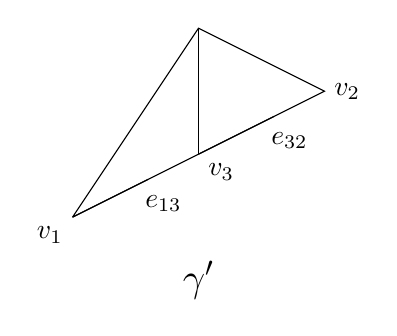
\begin{tikzpicture}[scale=0.8,]
					\node[below left] (v1) at (0,0) {$v_1$};
					\node[right] (v2) at (4,2) {$v_2$};
					\node[below right] (v3) at (2,1) {$v_3$};
					\node[below right] (e13) at (1,0.5) {$e_{13}$};
					\node[below right] (e32) at (3,1.5) {$e_{32}$};
					\draw[\myarrow] (0,0) -- (1.2,0.6);
					\draw[\myarrow] (2,1) -- (3.2,1.6);
					\draw (0,0) -- (4,2) -- (2,3) -- (0,0);
					\draw (2,1) -- (2,3);
					\node (gamma) at (2,-1) {{\Large $\gamma'$}};
				\end{tikzpicture}
				\caption{有偏序关系的图$\gamma$ 和 $\gamma'$}\label{figure-twogragh}
			\end{figure}

			为此,对于每一对图 $\gamma \prec \gamma'$ 引入图限制映射
			\begin{equation}
				p_{\gamma' \gamma} \colon \bar{\configurationspace{A}}_{\gamma'} \rightarrow \bar{\configurationspace{A}}_\gamma \qc h_{\gamma'} \mapsto \left.h_{\gamma'}\right|_{\gamma},
			\end{equation}
			它满足对于 $\gamma \prec \gamma' \prec 	\gamma''$ 有
			\begin{equation}
				p_{\gamma'' \gamma} = p_{\gamma' \gamma} \circ p_{\gamma'' \gamma'},
			\end{equation}
			则有
			\begin{equation}
				p_{\gamma' \gamma}\left( A_{\gamma'} \right) = A_\gamma,
			\end{equation}
			于是考虑如下定义
			\begin{Definition}
				投影系统(projective system)$\left\{ \bar{\configurationspace{A}}_\gamma, p_{\gamma' \gamma} \right\}$ 的\emph{投影极限}(projective limit)定义为 $\bar{\configurationspace{A}}_\infty$ 的一个子集
				\begin{equation}
					\varprojlim_{\gamma} \bar{\configurationspace{A}}_\gamma \definedby \left\{ {\left( h_\gamma \right)}_{\gamma \in \Gamma} \in \bar{\configurationspace{A}}_{\infty} \,\middle\vert\, p_{\gamma' \gamma}(h_{\gamma'}) = h_\gamma\qc \forall \gamma \prec \gamma' \right\}.
				\end{equation}
			\end{Definition}
			我们不加证明地列出以下结果:
			\begin{Property}
				\begin{enumerate}
					\item $p_{\gamma' \gamma}$ 都是连续满射;
					\item $\varprojlim_{\gamma} \bar{\configurationspace{A}}_\gamma$ 是 $\bar{\configurationspace{A}}_\infty$ 的闭子集,因而在子空间拓扑下也是紧致豪斯多夫空间;
					\item 映射
					\begin{equation}
						\Phi \colon \bar{\configurationspace{A}} \rightarrow \varprojlim_{\gamma} \bar{\configurationspace{A}}_\gamma \qc A \mapsto {\left( h_\gamma \definedby A|_\gamma \right)}_{\gamma \in \Gamma}
					\end{equation}
					是双射。
				\end{enumerate}
			\end{Property}
			至此,用 $\Phi$ 将 $\bar{\configurationspace{A}}$ 与 $\varprojlim_{\gamma} \bar{\configurationspace{A}}_\gamma$ 认同,即在 $\bar{\configurationspace{A}}$ 上定义了一个紧致豪斯多夫拓扑。

		\subsection{\texorpdfstring{$\bar{\configurationspace{A}}$上的测度}{量子位型空间上的测度}}

			上一节中为 $\bar{\configurationspace{A}}$ 定义的紧致豪斯多夫拓扑将对其上测度的定义起到很大帮助。本节定义 $\bar{\configurationspace{A}}$ 上的 Ashtekar-Lewandowski 测度,参见\cite{Ashtekar1994,Thiemann0210094,Thiemann2007}。

			考虑连续函数的集合 $C(\bar{\configurationspace{A}})$,根据 Riesz-Markov-Kakutani 表示定理,由于 $\bar{\configurationspace{A}}$ 具有紧致豪斯多夫拓扑,其上的正则 Borel 测度 $\mu$ 与 $C(\bar{\configurationspace{A}})$ 上的正定线性泛函 $\Lambda$ 通过下式一一对应
			\begin{equation}
				\Lambda(f) = \int_{\bar{\configurationspace{A}}} \dd{\mu} f \qc \forall f \in C(\bar{\configurationspace{A}}).
			\end{equation}
			注意到 $C(\bar{\configurationspace{A}})$ 上可定义上确界范数 $\norm{f} \definedby \sup_{A \in \bar{\configurationspace{A}}} \abs{f(A)}$,可以检验 $C(\bar{\configurationspace{A}})$ 构成 $C^*$-代数,则一个泛函分析中的标准结果是 $C(\bar{\configurationspace{A}})$ 上的线性泛函自动是连续的,因而有界,且 $\norm{\Lambda} = \Lambda(1)$,故我们总可以选择 $\Lambda$ 使 $\Lambda(1)=1$,则 $\mu$ 是一个概率测度。

			为了明确定义一个 $\Lambda$,考察柱函数与 $C(\bar{\configurationspace{A}})$ 的关系。这里重新定义一下 $\Cyl^k(\bar{\configurationspace{A}})$ 以代替之前在 $\configurationspace{A}$ 上定义的 $\Cyl^k$。
			\begin{Definition}
				取两个 $k$ 阶可微的函数 $f_\gamma \in C^k(\bar{\configurationspace{A}}_\gamma)$ 与 $f_{\gamma'} \in C^k(\bar{\configurationspace{A}}_{\gamma'})$\footnote{这里 $k$ 阶可微的定义是将 $\SU{2}^{\card{E(\gamma)}}$ 的光滑结构也搬到 $\bar{\configurationspace{A}}_\gamma$ 上定义的。},若它们满足任取 $\gamma''$ 使得 $\gamma , \gamma' \prec \gamma''$,有
				\begin{equation}
					p^*_{\gamma'' \gamma} f_\gamma = p^*_{\gamma'' \gamma'} f_{\gamma'},
				\end{equation}
				称 $f_\gamma$ 和 $f_{\gamma'}$ 是等价的,或 cylindrically consist,记为 $f_\gamma \sim f_{\gamma'}$。则定义 $\bar{\configurationspace{A}}$ 上的 $k$ 阶可微柱函数的集合为
				\begin{equation}
					\Cyl^k(\bar{\configurationspace{A}}) \definedby \left. \left( \bigcup_{\gamma \in \Gamma} C^k \left(\bar{\configurationspace{A}}_\gamma \right) \right) \middle/ \sim \right. ,
				\end{equation}
				特别地,有
				\begin{equation}
					\Cyl(\bar{\configurationspace{A}}) = \left. \left( \bigcup_{\gamma \in \Gamma} C\left(\bar{\configurationspace{A}}_\gamma\right) \right) \middle/ \sim \right. .
				\end{equation}
			\end{Definition}
			\begin{Remark}
				按照定义,每一个 $f_\gamma$ 可定义一个 $f= [f_\gamma] \in \Cyl^k(\bar{\configurationspace{A}})$;每一个 $f\in \Cyl^k(\bar{\configurationspace{A}})$ 都可找到合适的图 $\gamma$ 使 $f$ 有一个代表元 $f_\gamma$,即 $f=[f_\gamma]$;任取 $f,f' \in \Cyl^k(\bar{\configurationspace{A}})$,可找到一个图 $\gamma$ 及 $f_\gamma, f^\prime_\gamma \in C^k(\bar{\configurationspace{A}}_\gamma)$ 使得 $f=[f_\gamma],f'=[f^\prime_\gamma]$。
			\end{Remark}
			容易验证,$C^k(\bar{\configurationspace{A}}_\gamma)$ 上通常的加法、乘法、数乘和复共轭可良定义到 $\Cyl^k(\bar{\configurationspace{A}})$ 上,使其成为含幺阿贝尔 $*$-代数。在 $\Cyl(\bar{\configurationspace{A}})$ 上也可定义上确界范数,并完备化得 $\overline{\Cyl(\bar{\configurationspace{A}})}$,这是一个 $C^*$-代数,它正是 $C(\bar{\configurationspace{A}})$\cite{Thiemann2007}。
	
			于是我们现在知道,$C(\bar{\configurationspace{A}})$ 中的函数可视为 $\Cyl(\bar{\configurationspace{A}})$ 中的柯西列 $\left\{ [f_\gamma] \right\}$。而 $\Lambda$ 连续,故只需关注 $\Lambda$ 在柱函数上的取值。这里为了绕开关于投影极限上测度的定理,不按照 Ashtekar 和 Lewandowski \cite{Ashtekar1994} 及 \cite{Thiemann2007} 的方式继续推导,而是直接引入 spin-network 的概念:
			\begin{Definition}
				\begin{enumerate}
					\item 给定一个图 $\gamma$,对每条边 $e\in E(\gamma)$ 标记一组数 $(j_e,m_e,n_e)$,其中 $j_e$ 是取半正整数的自旋量子数,$m_e$,$n_e$ 是在 $\left\{ -j_e, -j_e+1, \cdots , j_e \right\}$ 中取值的磁量子数,则四元组
					\begin{equation}
						s \definedby \left( \gamma, \myvec{j} \definedby (j_e)_{e\in E(\gamma)}, \myvec{m} \definedby (m_e)_{e\in E(\gamma)}, \myvec{n} \definedby (n_e)_{e\in E(\gamma)} \right)
					\end{equation}
					称为一个\emph{自旋网络}(spin-network,简写为 SNW)。
					\item 记 Wigner D-矩阵
					\begin{equation}
						\tensor{D}{^j_m_n}(g) = \mel{jm}{\hat{\rho}_j(g)}{jn},
					\end{equation}
					其中 $\rho_j$ 是 $\SU{2}$ 的 spin-$j$ 不可约表示,则称
					\begin{equation}
						T_s \colon \bar{\configurationspace{A}} \rightarrow \mathbb{C} \qc A \mapsto \prod_{e\in E(\gamma)} \sqrt{2j_e + 1} \tensor{D}{^{j_e}_{m_e}_{n_e}}(A(e))
					\end{equation}
					为 $s$ 的 spin-network function(SNWF),并额外定义 $T_{(\emptyset, \myvec{0},\myvec{0},\myvec{0})} = 1$。
				\end{enumerate}
			\end{Definition}
			使用 SNWF 的动机之一是它们是互相线性独立的,而不像 Wilson loop 有 Mandelstam 恒等式互相联系。%由 Peter-Weyl 定理,$\tensor{\pi}{^j_m_n} = \sqrt{2j+1} \tensor{D}{^j_m_n}$ 构成 $L^2(\SU{2},\mu_H)$ 的一组正交归一基底,其中 $\mu_H$ 是哈尔测度(Haar measure),则某个图上面的所有 SNWF 构成 $L^2(\bar{\configurationspace{A}}_\gamma, \mu_H^{\card{E(\gamma)}})$ 的正交归一基,$\Span \left\{ T_{s} \right\}_{s=(\gamma,\cdot,\cdot,\cdot)}$ 在 $C(\bar{\configurationspace{A}}_\gamma)$ 中稠密。
			根据 Stone-Weierstrass 定理,$\Span\left\{ T_s \right\}$ 在 $C(\bar{\configurationspace{A}})$ 中稠密,所以只需关心 $\Lambda$ 在 SNWF 上的取值。以下定义 Ashtekar-Lewandowski 测度:
			\begin{Definition}
				Ashtekar-Lewandowski 测度 $\mu_{\text{A-L}}$ 由以下正定线性泛函唯一确定:
				\begin{equation}
					\Lambda_{\text{A-L}}(T_s) \definedby
					\begin{cases}
						1, & s=(\emptyset,\myvec{0},\myvec{0},\myvec{0}),\\
						0, & \text{otherwise}.
					\end{cases}
				\end{equation}
			\end{Definition}
			于是可定义 $\Hkin \definedby L^2(\bar{\configurationspace{A}},\mu_{\text{A-L}})$。

			可以通过群表示的计算证明:
			\begin{Property}
				\begin{enumerate}
					\item SNWF 构成 $\Hkin$ 的一组正交归一基底。
					\item 任取 $f=[f_\gamma] \in \Cyl(\bar{\configurationspace{A}})$,有
					\begin{equation}
						\int_{\bar{\configurationspace{A}}} \dd{\mu_{\text{A-L}}} f = \Lambda_{\text{A-L}}(f) = \int_{\SU{2}^{\card{E(\gamma)}}} \left( \prod_{e\in E(\gamma)} \dd{\mu_H}(h_e) \right) f_\gamma(h_{e_1}, \cdots, h_{e_{\card{E(\gamma)}}}),
					\end{equation}
					特别地,任取 $f=[f_\gamma]$,$f'=[f^\prime_\gamma]$,
					\begin{equation}
						\begin{split}
							&\ip{f}{f'}_{\text{kin}} \definedby \int_{\bar{\configurationspace{A}}} \dd{\mu_{\text{A-L}}} \bar{f} f'\\
							={}& \int_{\SU{2}^{\card{E(\gamma)}}} \left( \prod_{e\in E(\gamma)} \dd{\mu_H}(h_e) \right) \overline{f_\gamma(h_{e_1}, \cdots, h_{e_{\card{E(\gamma)}}})}f^\prime_\gamma(h_{e_1}, \cdots, h_{e_{\card{E(\gamma)}}}).
						\end{split}
					\end{equation}
				\end{enumerate}
			\end{Property}
			由于 $\bar{\configurationspace{A}}_\gamma$ 与 $\SU{2}^{\card{E(\gamma)}}$ 认同,不妨记 $\mu_\gamma$ 为测度
			\begin{equation}
				\int_{\bar{\configurationspace{A}}_\gamma} \dd{\mu_\gamma} f_\gamma = \Lambda_\gamma(f_\gamma) \definedby \int_{\SU{2}^{\card{E(\gamma)}}} \left( \prod_{e\in E(\gamma)} \dd{\mu_H}(h_e) \right) f_\gamma(h_{e_1}, \cdots, h_{e_{\card{E(\gamma)}}}),
			\end{equation}
			并定义
			\begin{equation}
				\Hil_\gamma \definedby L^2(\bar{\configurationspace{A}}_\gamma,\mu_\gamma) = L^2 \left(\SU{2}^{\card{E(\gamma)}}, \mu_H^{\card{E(\gamma)}} \right) = \otimes^{\card{E(\gamma)}} L^2(\SU{2}, \mu_H),
			\end{equation}
			将 $e\in E(\gamma)$ 也看作图,又有 $\Hil_e = L^2(\bar{\configurationspace{A}}_e,\mu_e) = L^2(\SU{2}, \mu_H)$,则又有 $\Hil_\gamma = \bigotimes_{e\in E(\gamma)} \Hil_e$。还有一个有用的结果是
			\begin{Property}
				\begin{equation}
					\Hkin = \left\langle \Cyl\left( \bar{\configurationspace{A}} \right) \right\rangle = \left\langle \bigcup_{\gamma \in \Gamma} \Hil_\gamma \right\rangle,
				\end{equation}
				其中 $\left\langle \cdot \right\rangle$ 表示对于 $\ip{\cdot}_{\text{kin}}$ 取完备化。
			\end{Property}
			因此,我们常常能把 $\Hkin$ 上的问题转变为 $\Hil_\gamma$ 上的问题,而后者直观得多。

		\subsection{\texorpdfstring{$\staralgebra{B}$ 在 $\Hkin$ 上的表示}{B 在希尔伯特空间 H 上的表示}}

			本节定义 $\staralgebra{B}$ 在 $\Hkin$ 上唯一的不可约表示。此表示的严格定义及唯一性的证明参见 \cite{Thiemann2007}。

			按照定义 $\Cyl^k(\bar{\configurationspace{A}})$ 的方式,可在 $\left\{ V^k\left(\bar{\configurationspace{A}}_\gamma\right) \cong V^k\left(\SU{2}^{\card{E(\gamma)}}\right) \right\}_{\gamma\in \Gamma}$ 上定义等价关系 $\sim$,并定义
			\begin{equation}
				V^k\left( \bar{\configurationspace{A}} \right) \definedby \left. \left( \bigcup_{\gamma\in \Gamma} V^k\left( \bar{\configurationspace{A}}_\gamma \right) \right) \middle/ \sim \right. ,
			\end{equation}
			这里只需知道 $v^i_S \in V^\infty\left( \bar{\configurationspace{A}} \right)$。选择 $\Dkin \definedby \Cyl^\infty \left( \bar{\configurationspace{A}} \right)$,定义由下式确定的表示
			\begin{equation}
				\begin{split}
					\left( \pi(f)f' \right)(A) &\definedby (f f')(A),\\
					\left( \pi\left(v^i_S\right) f \right)(A) &\definedby \ii\hbar \left( v^i_S(f) \right)(A),\\
					\pi(a) &\definedby \pi(f) + \pi\left(v^i_S\right),
				\end{split}
			\end{equation}
			其中 $f,f'\in \Cyl^\infty\left(\bar{\configurationspace{A}}\right)$,$v^i_S = \left\{ P_i(S), \cdot \right\} \in V^\infty \left( \bar{\configurationspace{A}} \right)$,$a=\left( f, v^i_S \right) \in \staralgebra{B}$。则容易验证
			\begin{equation}
				\left[ \pi(a), \pi(b) \right] = \pi\left( \left[ a,b \right] \right).
			\end{equation}
			对于 $*$-运算,首先容易验证 $\pi(f)^\dagger = \pi(\bar{f})$;$\bar{v}^i_S = v^i_S$,而由~\eqref{eq-flux_function_algebra} 知
			\begin{equation}
				\pi\left(v^i_S\right) = \frac{\hbar}{2} \sum_{v\in V(S) \cap S} \left( \sum_{e:v\in e} \kappa(S,e) \hat{J}^{(e,v)}_i \right),\label{eq-flux_operator}
			\end{equation}
			其中 $v\in e$ 表示 $v$ 是 $e$ 的端点,而 $\hat{J}^{(e,v)}_i$ 的定义如下,先定义 $\Hil_e = L^2(\SU{2},\mu_H)$ 上的两个角动量算符
			\begin{equation}
				\hat{J}^{(L)}_i \definedby \ii L_i \qc \hat{J}^{(R)}_i \definedby \ii R_i,
			\end{equation}
			其中 $L_i$ 和 $R_i$ 是左不变和右不变矢量场。容易检查它们自伴。对于 $\Hil_\gamma = \bigotimes_{e\in E(\gamma)} \Hil_e$,任取 $v\in V(\gamma)$,$e\in E(\gamma)$,定义
			\begin{equation}
				\hat{J}^{(e,v)}_i \definedby
				\begin{cases}
					\ii L^{(e)}_i, & v=s(e),\\
					\ii R^{(e)}_i, & v=t(e),\\
					0, & \text{else},
				\end{cases}
			\end{equation}
			其中 $L_i^{(e)}$ 和 $R_i^{(e)}$ 是~\eqref{eq-invariance_vector_field} 中定义的左不变和右不变矢量场。$\hat{J}^{(e,v)}_i$ 可以被写为
			\begin{equation}
				\hat{J}^{(e,v)}_i =
				\begin{cases}
					\hat{\II} \otimes \cdots \otimes \hat{J}_i^{(L)} \otimes \cdots \otimes \hat{\II}, & v=s(e),\\
					\hat{\II} \otimes \cdots \otimes \hat{J}_i^{(R)} \otimes \cdots \otimes \hat{\II}, & v=t(e),\\
					0, & \text{else},
				\end{cases}
			\end{equation}
			则它显然是自伴的。于是由~\eqref{eq-flux_operator} 知 $\pi\left(v^i_S\right)$ 自伴。故 $\pi$ 保泊松括号、$*$-运算,它的确是一个表示。
			\begin{Theorem}
				表示 $\pi$ 是 $\staralgebra{B}$(的泛包络代数$\staralgebra{A}$)的不可约表示,且在一定的限制条件下有唯一性。
			\end{Theorem}
			% \begin{Proof}
			% 	这里证明 $\pi$ 的不可约。由于 $\bar{\configurationspace{A}}$ 紧致,$f$ 必有界,故 $\pi(f)$ 是有界算子,它实际上定义在整个 $\Hkin = L^2(\bar{\configurationspace{A}},\mu_{\text{A-L}})$。令 $\Omega = 1 \in \Cyl^\infty(\bar{\configurationspace{A}})$,则 $\pi(f) \Omega = f$ 即跑遍 $\Hkin$ 的一个稠密子空间 $\Dkin = \Cyl^\infty(\bar{\configurationspace{A}})$,故 $\Omega$ 是 cyclic vector。再任取 $\psi \in \Hkin$,$\pi$ 不可约。
			% \end{Proof}
	\section{约束算符的求解}

		本节将在量子理论中求解约束~\eqref{eq-constrains_in_Ashtekar_connection}:
		\begin{equation*}
			\begin{split}
				\tensor{G}{_i} &= \AD{a} \tensor{\tilde{P}}{^a_i} = \Partial{a} \tensor{\tilde{P}}{^a_i} + \tensor{\vol}{_i_j^k} \tensor{A}{^j_a} \tensor{\tilde{P}}{^a_k},\\
				\tensor{V}{_a} &= \tensor{\tilde{P}}{^b_i} \tensor{F}{^i_a_b} - \frac{1+\gamma^2}{\gamma} \tensor{K}{^i_a} \tensor{G}{_i},\\
				C &= \frac{\gkappa \gamma^2}{2\sqrt{\abs{\det h}}} \tensor{\tilde{P}}{^a_i} \tensor{\tilde{P}}{^b_j} \left[ \tensor{\vol}{^i^j_k} \tensor{F}{^k_a_b} - \left( 1+ \gamma^2 \right) \tensor{K}{^i_a} \wedge \tensor{K}{^j_b} \right]\\
				& \qquad + \gkappa \left( 1 +\gamma^2 \right) \tensor{G}{^i} \Partial{a} \left( \frac{\tensor{\tilde{P}}{^a_i}}{\sqrt{\abs{\det h}}} \right).
			\end{split}
		\end{equation*}
		回忆它们的约束代数~\eqref{eq-constrain_algebra},我们曾经提起过高斯约束构成双边理想,可以先独立解出,而且能直接在 $\Hkin$ 上求解得到 $\SU{2}$ 不变空间 $\Hkin^0$,较为简单。之后将以 $\Hkin^0$ 为 kinematical 希尔伯特空间,继续求解其他约束。
		
		\subsection{量子高斯约束}
		
			在~\eqref{eq-smeared_Gauss_constrain} 中定义了经典的 smeared 高斯约束
			\begin{equation}
				G(\Lambda) = \int_{\spc} \dd[3]{x} \tensor{\Lambda}{^i} \AD{a} \tensor{\tilde{P}}{^a_i} = - \int_{\spc} \dd[3]{x} \tensor{\tilde{P}}{^a_i} \AD{a} \tensor{\Lambda}{^i},
			\end{equation}
			这是动量在3维的smear,将 $\int_{\spc} \dd[3]{x} \tensor{\tilde{P}}{^a_i} \AD{a} \tensor{\Lambda}{^i}$ 记为 $P(\ADd \Lambda)$,并定义 $\bar{\configurationspace{A}}$ 上的矢量场
			\begin{equation}
				Y_{\ADd \Lambda}([f_\gamma]) \definedby \left\{ - P(\ADd \Lambda), f_\gamma \right\},
			\end{equation}
			则高斯约束可自然被量子化为
			\begin{equation}
				\begin{split}
					\hat{G}(\Lambda) f &\definedby \ii\hbar Y_{\ADd \Lambda}(f)\\
					&= \hbar \sum_{v\in V(\gamma)} \tensor{\Lambda}{^i}(v) \hat{J}^v_i f_\gamma,
				\end{split}
			\end{equation}
			其中
			\begin{equation}
				\hat{J}^v_i \definedby \sum_{e:v\in e} \hat{J}^{(e,v)}_i,
			\end{equation}
			于是根据群表示的知识,$\hat{G}(\Lambda)$ 具有点谱,是可以直接在 $\Hkin$ 上求解的,量子高斯约束方程是
			\begin{equation}
				\hat{J}^v_i f_\gamma =0\qc \forall v \in V(\gamma),
			\end{equation}
			或等价地
			\begin{equation}
				\left( \hat{J}^v \right)^2 f_\gamma =0\qc \forall v \in V(\gamma),
			\end{equation}
			其中 $\left( \hat{J}^v \right)^2 \definedby \tensor{\delta}{^i^j} \hat{J}^v_i \hat{J}^v_j$。
		
			为了求解量子高斯约束方程,我们重新观察之前构造的 $\Hkin$ 的一组基底——spin-network function。注意到 $\Hil_\gamma = \bigotimes_{e\in E(\gamma)} \Hil_e$,而 $\Hil_e \cong L^2(\SU{2},\mu_H)$ 上 $\left\{ \hat{J}^2, \hat{J}^{(L)}_3, \hat{J}^{(R)}_3 \right\}$ 构成完备对易算符集,其中
			\begin{equation}
				\hat{J}^2 \definedby \tensor{\delta}{^i^j} \hat{J}^{(L)}_i \hat{J}^{(L)}_j \equiv \tensor{\delta}{^i^j} \hat{J}^{(R)}_i \hat{J}^{(R)}_j
			\end{equation}
			它们的共同本征态就是 $\tensor{\pi}{^j_m_n}$:
			\begin{equation}
				\hat{J}^2 \tensor{\pi}{^j_m_n} = j(j+1) \tensor{\pi}{^j_m_n} \qc \hat{J}^{(L)}_3 \tensor{\pi}{^j_m_n} = m \tensor{\pi}{^j_m_n} \qc \hat{J}^{(R)}_3 \tensor{\pi}{^j_m_n} = n \tensor{\pi}{^j_m_n},
			\end{equation}
			故以 $\tensor{\pi}{^j_m_n}$ 为基底就是在算符集 $\left\{ \hat{J}^2, \hat{J}^{(L)}_3, \hat{J}^{(R)}_3 \right\}$ 下分解 $\Hil_e$。这可以通过 $\tensor{\pi}{^j_m_n}(g) = \mel{jm}{\hat{\rho}^j(g)}{jn} = \tr(\op{jn}{jm}\hat{\rho}^j(g))$ 从另一方面理解,映射
			\begin{equation}
				\op{jn}{jm} \mapsto \tensor{\pi}{^j_m_n} = \tr(\op{jn}{jm}\hat{\rho}^j(\cdot))
			\end{equation}
			是 $\bigoplus_j \left( \Hil_j \otimes \Hil_j^* \right)$ 到 $\Hil_e$ 的同构,其中 $\Hil_j$ 是 $\SU{2}$ 的 spin-$j$ 表示空间。$\hat{J}^{(L)}_i$ 可理解为作用在左矢 $\bra{jm}$,即是 $\Hil_j^*$ 上的角动量算符,而 $\hat{J}^{(R)}_i$ 可理解为作用在右矢 $\ket{jn}$,即是 $\Hil_j$ 上的角动量算符。
			于是 spin-network function 作为 $\tensor{\pi}{^j_m_n}$ 的张量积,是完备对易算符集 $\left\{ \left( \hat{J}^{(e)} \right)^2, \hat{J}^{(e,s(e))}_3, \hat{J}^{(e,t(e))}_3 \right\}_{e\in E(\gamma)}$ 的共同本征函数,对应于分解
			\begin{equation}
				\begin{split}
					\Hil_\gamma &= \bigotimes_{e\in E(\gamma)} \Hil_e = \bigotimes_{e\in E(\gamma)} \left( \bigoplus_{j_e} \left( \Hil^{(e)}_{j_e} \otimes \Hil^{(e)*}_{j_e} \right) \right)\\
					&= \bigoplus_{\myvec{j}} \left( \bigotimes_{e\in E(\gamma)} \left( \Hil^{(e)}_{j_e} \otimes \Hil^{(e)*}_{j_e} \right) \right),\label{eq-spin_network_function_decompose}
				\end{split}
			\end{equation}
			量子高斯约束算符中的 $\hat{J}^v_i = \sum_{e:v\in e} \hat{J}^{(e,v)}_i$ 提示我们在顶点处进行角动量耦合。定义
			\begin{equation}
				\Hil_j^{(e,v)} \definedby
				\begin{cases}
					\Hil_j, & v=t(e),\\
					\Hil_j^*, & v=s(e),\\
					\left\{ 0 \right\}, & \text{otherwise},
				\end{cases}
			\end{equation}
			则可继续改写
			\begin{equation}
				\begin{split}
					\Hil_\gamma &= \bigoplus_{\myvec{j}} \left( \bigotimes_{e\in E(\gamma)} \left( \bigotimes_{\substack{v:v\in e}} \Hil_{j_e}^{(e,v)} \right) \right) = \bigoplus_{\myvec{j}} \left( \bigotimes_{v\in V} \left( \bigotimes_{\substack{e:v\in e}} \Hil_{j_e}^{(e,v)} \right) \right),
				\end{split}
			\end{equation}
			顶点 $v$ 处的张量积表示 $\bigotimes_{\substack{e:v\in e}} \Hil_{j_e}^{(e,v)}$ 就是 $\hat{J}_i^{v}$ 作用的空间,可分解为不可约表示的直和
			\begin{equation}
				\bigotimes_{\substack{e:v\in e}} \Hil_{j_e}^{(e,v)} = \bigoplus_{l} \Hil_{\myvec{j}(v),l_v}^{v},
			\end{equation}
			其中 $l_v$ 是 $\left( \hat{J}^{v} \right)^2$ 的量子数,$\myvec{j}(v) = \left( j_e \right)_{v\in e}$ 是所有以 $v$ 为端点的边上标记的 $j_e$ 的数组。故
			\begin{equation}
				\Hil_\gamma = \bigoplus_{\myvec{j}} \left( \bigoplus_{\myvec{l}} \left( \bigotimes_{v\in V(\gamma)} \Hil_{\myvec{j}(v),l_v}^{v} \right) \right),
			\end{equation}
			则 $\Hil_\gamma$ 中量子高斯约束的解空间即为
			\begin{equation}
				\Hil_\gamma^0 \definedby \bigoplus_{\myvec{j}} \left( \bigotimes_{v\in V(\gamma)} \Hil_{\myvec{j}(v),l_v=0}^{v} \right),\label{eq-H0gamma_decompose}
			\end{equation}
			注意到
			\begin{equation}
				\Hil_{\myvec{j}(v),l_v=0}^{v} = \Inv\left( \bigotimes_{\substack{e:v\in e}} \Hil_{j_e}^{(e,v)} \right)
			\end{equation}
			是数学中所说的 intertwiner space,可依照分解式~\eqref{eq-H0gamma_decompose} 给出 $\Hil_\gamma^0$ 的一组基底:
			\begin{Definition}
				任给定图 $\gamma$,指定 $\myvec{j} = \left( j_e \right)_{e\in E(\gamma)}$,使得每个顶点处 $\bigotimes_{\substack{e:v\in e}} \Hil_{j_e}^{(e,v)}$ 都存在 intertwiner;然后对每个顶点指定一个 intertwiner $i_v \in \Hil_{\myvec{j}(v),l_v=0}^{v}$,记规范不变的spin-network 为 $s=(\gamma,\myvec{j},\myvec{i})$,则定义\emph{spin-network state}为
				\begin{equation}
					\psi_s(A) \definedby \operatorname{C} \left( \bigotimes_{v\in V(\gamma)} i_v \bigotimes_{e\in E(\gamma)} \rho^j(A(e)) \right),
				\end{equation}
				其中 $\operatorname{C}(\cdot)$ 指对每一对 $(e,v)$ 将 intertwiner $i_v$ 与 $\rho^j(A(e))$ 相对应的指标缩并。
		
				当 $\myvec{j}$ 取遍且 $i_v$ 取遍 intertwiner space 取定的一组基底时,spin-network state 构成 $\Hil_\gamma^0$ 的基底。
			\end{Definition}
			对于整个 $\Hkin$,则需要一些新定义和一个分解定理\cite{Han2005}:
			\begin{Definition}
				对图 $\gamma$,若 $v\in V(\gamma)$ 满足:以 $v$ 为顶点的边有且只有两条,且都不是以 $v$ 为基点的圈(loop),即都只过 $v$ 一次,并且它们相乘($\circ$运算)是解析的,则称 $v$ 为\emph{伪顶点}。换句话说,伪顶点人为地将一条边分为两条。
				
				定义
				\begin{equation}
					\Hil_\gamma^\prime = \bigoplus_{\left( \myvec{j},\myvec{l} \right) \in I_\gamma} \left( \bigotimes_{v\in V(\gamma)} \Hil_{\myvec{j}(v),l_v}^{v} \right),
				\end{equation}
				其中 $I_\gamma$ 对 $\myvec{j}$ 和 $\myvec{l}$ 作如下两条限定:所有 $j_e \neq 0$;对每个伪顶点,$l\neq 0$。
			\end{Definition}
			\begin{Theorem}
				$\Hkin$ 有直和分解
				\begin{equation}
					\Hkin = \left( \bigoplus_{\gamma \in \Gamma} \Hil_\gamma^\prime \right) \oplus \mathbb{C}.
				\end{equation}
			\end{Theorem}
			每个 $\Hil_\gamma^\prime$ 不过是对 $\left( \myvec{j}, \myvec{l} \right)$ 作限制,对量子高斯约束方程没有影响,故在 $\Hil_\gamma^\prime$ 中的规范不变子空间为
			\begin{equation}
				\Hil_\gamma^{0\prime} = \bigoplus_{\left( \myvec{j},\myvec{l}=\myvec{0} \right) \in I} \left( \bigotimes_{v\in V(\gamma)} \Hil_{\myvec{j}(v),l_v=0}^{v} \right),
			\end{equation}
			$\Hil_\gamma^{0\prime}$ 的基底也只需对 spin-network state 的 $\myvec{j}$ 作出限制即可。于是可直接得到
			\begin{Theorem}
				高斯约束的解子空间为
				\begin{equation}
					\Hkin^0 = \left( \bigoplus_{\gamma \in \Gamma} \Hil_\gamma^{0\prime} \right) \oplus \mathbb{C},
				\end{equation}
				其上的一组基底是
				\begin{equation}
					\left\{ \psi_{s=(\gamma,\myvec{j},\myvec{i})} \,\middle|\, (\myvec{j},\myvec{0}) \in I_\gamma, \text{每个 $i_v$ 在取定的一组基底中取值}, \gamma\in \Gamma \right\}.
				\end{equation}
			\end{Theorem}		
